\documentclass[12pt]{report}

\usepackage[a4paper,margin=1in]{geometry}
\usepackage[T1]{fontenc}
\usepackage{graphicx}
\usepackage{amsmath}
\usepackage{listings}
\usepackage{xcolor}
\usepackage{hyperref}
\usepackage{float}
\usepackage{booktabs}
\usepackage[numbers]{natbib}
\usepackage{setspace}
\usepackage{algorithm}
\usepackage{algpseudocode}
\usepackage{pgfplots}
\pgfplotsset{compat=1.17}

\begin{document}

\begin{titlepage}

\begin{center}

\vspace*{1.5cm}

%------------------------------------------------
% University Logo
%------------------------------------------------


\includegraphics[width=0.18\textwidth]{bamberg_logo.png}

\vspace{0.3cm}

{\Large \textcolor{brown}{\textsc{Bamberg University}}}

\vspace{1.8cm}

{\large \textsc{Master Thesis}}

\vspace{1cm}

\noindent\rule{0.75\textwidth}{0.5pt}

\vspace{0.7cm}

{\Huge \bfseries
Higher-Order SQL Lambda Functions in DuckDB\\[0.5cm]
\large Design, Implementation, and Evaluation of Forward-Mode and Reverse-Mode Automatic Differentiation
}

\vspace{0.7cm}

\noindent\rule{0.75\textwidth}{0.5pt}

\vspace{2cm}

%------------------------------------------------
% Author and Supervisor
%------------------------------------------------

\begin{minipage}{0.4\textwidth}
\begin{flushleft}
\textit{Author:}\\
Lakshmi Nair
\end{flushleft}
\end{minipage}
\hfill
\begin{minipage}{0.4\textwidth}
\begin{flushright}
\textit{Supervisor:}\\
Prof.\ Dr.\ Maximilian E.\ Sch\"ule
\end{flushright}
\end{minipage}

\vfill

%------------------------------------------------
% Submission Text
%------------------------------------------------

\begin{spacing}{1.1}
\textit{
A thesis submitted in fulfillment of the requirements\\
for the degree of Master of Science in International Software Systems Science\\
in the
}
\end{spacing}

\vspace{0.5cm}

Chair of Data Engineering\\
Faculty Information Systems and Applied Computer Sciences

\vfill

May 2026

\end{center}

\end{titlepage}


\newpage

%------------------------------------------------
% Quote Page
%------------------------------------------------

\vspace*{4cm}

\begin{flushright}
\textit{
``The most powerful systems are those that allow us\\
to express complex ideas with simple abstractions.''
}
\\[1cm]
--- John Ousterhout
\end{flushright}

\newpage


%------------------------------------------------
% Abstract
%------------------------------------------------

\chapter*{Abstract}
\addcontentsline{toc}{chapter}{Abstract}

Modern analytical workflows increasingly combine relational data processing with
machine learning, yet the two are typically separated: data is extracted from the
database, gradients and models are computed in external frameworks, and results
are written back. This separation causes unnecessary data movement and prevents
the database from optimizing the combined workload. Automatic differentiation
(AD), the technique underlying gradient-based machine learning, is not natively
supported by relational database systems.

This thesis investigates whether automatic differentiation can be integrated
directly into a modern analytical database system using higher-order SQL lambda
expressions. The work is carried out in DuckDB, a high-performance in-process
analytical database optimized for vectorized execution. Lambda expressions,
which DuckDB supports as higher-order SQL functions, are treated as
differentiable programs: a lambda passed to an AD function is compiled into an
internal representation from which gradients are computed automatically, without
manual derivation. Both forward-mode and reverse-mode AD are designed and
implemented, and both return the full gradient of the lambda expression in a
single call. The implementation is integrated into DuckDB's binder and scalar
function subsystem and reuses the existing vectorized execution engine,
requiring only localized modifications to the database.

The implementation is evaluated on linear regression gradient-descent workloads
across dataset sizes ranging from one thousand to fifty thousand tuples,
comparing handwritten SQL gradients, forward-mode AD, and reverse-mode AD on an
optimized release build with single-threaded execution. Reverse-mode AD stays
within roughly $1.3\times$ to $2.2\times$ of the handwritten SQL baseline
across the evaluated dataset sizes, whereas forward-mode AD is slower, with
the gap between the two AD modes widening from roughly $1.5\times$ at one
thousand tuples to roughly $6.1\times$ at fifty thousand tuples. Forward-mode
AD performance was substantially improved by moving per-row string-based
operator dispatch to a bind-time hash-map cache, mirroring the design of the
reverse-mode instruction tape. The thesis demonstrates that differentiable
computation can be expressed and executed directly inside SQL queries, and
that bind-time compilation --- of the reverse-mode tape and of the
forward-mode operator cache --- is an effective optimization strategy for
automatic differentiation in a database engine.


\newpage

%------------------------------------------------
% Acknowledgements
%------------------------------------------------

\chapter*{Acknowledgements}
\addcontentsline{toc}{chapter}{Acknowledgements}

I would like to express my deepest gratitude to my thesis supervisor, Professor Dr.\ Maximilian E.\ Sch\"ule, for his invaluable guidance, continuous support, and insightful feedback throughout this research. His expertise in database systems greatly shaped the direction and quality of this work.

Special thanks go to the DuckDB development team and open-source community for creating an exceptional analytical database system. Their clean codebase and comprehensive documentation made this implementation possible.

I would also like to thank Maha M H Alwahibi and the researchers in the database systems group for the stimulating discussions, technical insights, and collaborative environment that enriched my understanding of the field.

I am deeply grateful to my family for their unconditional love, patience, and encouragement throughout my academic journey. Their belief in me has been my greatest source of strength and motivation.

Finally, I would like to thank my friends and colleagues who provided both technical assistance and emotional support during the challenging phases of this research.

\newpage


%------------------------------------------------
% Table of Contents
%------------------------------------------------

\tableofcontents
\newpage

%------------------------------------------------
% List of Figures
%------------------------------------------------

\listoffigures
\addcontentsline{toc}{chapter}{List of Figures}

\newpage

%------------------------------------------------
% List of Tables
%------------------------------------------------

\listoftables
\addcontentsline{toc}{chapter}{List of Tables}

\newpage

%------------------------------------------------
% List of Abbreviations
%------------------------------------------------

\chapter*{List of Abbreviations}
\addcontentsline{toc}{chapter}{List of Abbreviations}


\begin{tabular}{ll}
AD    & Automatic Differentiation \\
API   & Application Programming Interface \\
AST   & Abstract Syntax Tree \\
CPU   & Central Processing Unit \\
DBMS  & Database Management System \\
ML    & Machine Learning \\
OLAP  & Online Analytical Processing \\
RDBMS & Relational Database Management System \\
SIMD  & Single Instruction Multiple Data \\
SQL   & Structured Query Language \\
\end{tabular}


\newpage


%------------------------------------------------
% Main Content
%------------------------------------------------

%%%%%%%%%%%%%%%%%%%%%%%%%%%%%%%%%%%%%%%%%%%%%%%%%%%%
% CHAPTER 1 — INTRODUCTION
%%%%%%%%%%%%%%%%%%%%%%%%%%%%%%%%%%%%%%%%%%%%%%%%%%%%

\chapter{Introduction}
\label{ch:introduction}

\section{Background and Motivation}

The interaction between database systems and machine learning workflows has
grown substantially in recent years. Relational database management systems
(RDBMS) have long provided efficient mechanisms for structured data storage and
querying~\cite{codd1970relational,selinger1979access}, while modern machine
learning frameworks---such as TensorFlow~\cite{abadi2016tensorflow},
PyTorch~\cite{paszke2019pytorch}, JAX~\cite{jax2018}, and
MXNet~\cite{chen2015mxnet}---excel at gradient-based optimization and numerical
computation.

In real-world analytical pipelines these two worlds remain largely separate. A
typical workflow extracts data from the database, loads it into Python or R,
trains a model in an external framework, and finally writes the results back.
The cost of this round trip is felt at every stage: data must be moved across
process and language boundaries, the analytical pipeline is fragmented across
several tools, work is duplicated between the database and the framework, and
the database itself loses the opportunity to optimize the combined workload as a
single query. These limitations motivate the integration of automatic
differentiation (AD) directly inside SQL and the database engine.

\section{Automatic Differentiation}

Automatic differentiation computes derivatives by applying the chain rule at the
operation level~\cite{baydin2017automatic,griewank2008evaluating}. It comes in
two main forms. Forward-mode AD propagates derivatives alongside primal values
during expression evaluation, using dual-number arithmetic to carry a partial
derivative through every operation. Reverse-mode AD records the sequence of
operations during a forward pass and then propagates adjoint values back through
that record to produce the gradient with respect to every input.

Reverse-mode AD powers deep learning frameworks~\cite{pearlmutter2008reverse}
such as TensorFlow~\cite{abadi2016tensorflow}, PyTorch~\cite{paszke2019pytorch},
and JAX~\cite{jax2018}. It is the computational basis of gradient-based
optimizers, including stochastic gradient descent and adaptive methods such as
Adam~\cite{kingma2015adam}, and of more advanced uses of the gradient signal
such as gradient-based hyperparameter optimization~\cite{maclaurin2015reversible}.
No relational database currently supports AD natively.

\section{Why AD in SQL?}

Embedding AD inside SQL changes where gradients are computed and what users have
to do to obtain them. Gradients are computed where the data lives, so analytics
and machine learning share a single pipeline and a single execution engine;
gradient-descent loops can be expressed directly in SQL; and the database is
free to optimize the combined computation rather than treating it as an opaque
external step.

The primary objective of the proposed system is not to outperform handwritten
SQL gradients, but to automate gradient computation directly inside the database
system. Manual derivation of SQL gradients becomes increasingly difficult and
error-prone for complex analytical workloads. Automatic differentiation lets
users express differentiable computations declaratively using lambda expressions
while preserving database-native execution.

Prior systems such as MADlib~\cite{madlib}, Bismarck~\cite{feng2012unified},
and SystemML~\cite{boehm2013systemml} support in-database analytics, but still
require manually derived gradients or predefined model templates.
DuckDB~\cite{duckdb2019} supports higher-order functions and vectorized
execution~\cite{raasveldt2022modular}, making it suitable for AD integration.

\section{DuckDB and Higher-Order Lambdas}

DuckDB supports lambda expressions such as \verb|(x -> x * x + 3)|. These treat
expressions as first-class functions, which enables automatic differentiation
over them: the lambda body is precisely the differentiable program whose
gradient the AD system needs to compute.

\section{Problem Statement}

SQL on its own lacks the building blocks required for automatic differentiation.
There is no notion of a computation graph, no mechanism for propagating
derivatives through arithmetic operators, no place to store the intermediate
values that reverse-mode AD relies on, and no AD-capable operators in the scalar
function library. To address this, this thesis implements forward-mode AD using
dual-number propagation, reverse-mode AD using a compiled instruction tape, and
a bind-time tape compilation optimization that ensures the tape is built once
per query and reused for every row.

\section{Research Questions}

This thesis investigates whether automatic differentiation can be efficiently
integrated into a modern analytical database system using higher-order SQL
lambda expressions. The research focuses on the following questions:

\begin{enumerate}
  \item Can higher-order SQL lambda expressions be used to represent
        differentiable computations inside DuckDB?
  \item How can forward-mode and reverse-mode automatic differentiation be
        integrated into DuckDB's query execution pipeline?
  \item Can reverse-mode AD be optimized using bind-time tape compilation and
        reuse?
  \item What performance overhead is introduced by automatic differentiation
        inside SQL queries?
  \item Can vectorized execution in DuckDB efficiently support gradient
        computation over relational data?
\end{enumerate}

These research questions guide both the implementation and the experimental
evaluation presented throughout this thesis.

\section{Thesis Contributions}

The primary contributions of this thesis are summarized as follows:

\begin{itemize}
  \item Implementation of forward-mode automatic differentiation inside DuckDB
        using higher-order SQL lambda functions.
  \item Implementation of reverse-mode automatic differentiation with
        computation tape reuse.
  \item Integration of AD into DuckDB's binder and scalar function subsystem.
  \item Experimental evaluation comparing handwritten SQL gradients,
        forward-mode AD, and reverse-mode AD.
\end{itemize}

\section{Thesis Structure}

The remainder of the thesis is structured as follows. Chapter~\ref{ch:background}
introduces the background on automatic differentiation, differentiable
programming, and machine learning inside database systems. Chapter~\ref{ch:design}
describes DuckDB's architecture and the system design used to integrate AD into
its query pipeline. Chapter~\ref{ch:implementation} presents the implementation
of forward-mode and reverse-mode AD. Chapter~\ref{ch:evaluation} evaluates the
implementation on linear regression workloads. Chapter~\ref{ch:conclusion}
discusses the results, summarizes the contributions, and outlines future work.


%%%%%%%%%%%%%%%%%%%%%%%%%%%%%%%%%%%%%%%%%%%%%%%%%%%%
% CHAPTER 2 — Background & Related work
%%%%%%%%%%%%%%%%%%%%%%%%%%%%%%%%%%%%%%%%%%%%%%%%%%%%

\chapter{Background and Related Work}
\label{ch:background}

This chapter discusses the background concepts required for this thesis. The work combines ideas from automatic differentiation, differentiable programming, higher-order SQL functions, and database query execution. Since the implementation was developed inside DuckDB, this chapter also discusses vectorized query execution and machine learning inside database systems.

\section{Automatic Differentiation}

Automatic differentiation (AD) is a technique for computing exact derivatives of functions represented as programs. Unlike symbolic differentiation, AD does not manipulate mathematical expressions directly. Instead, it applies the chain rule during program execution.

Baydin et al.~\cite{baydin2017automatic} provide a detailed survey of AD methods and their applications in machine learning systems. Griewank and Walther~\cite{griewank2008evaluating} formally describe forward-mode and reverse-mode AD and explain how gradients can be propagated through computation graphs. Beyond the first-order gradient, the same operation-level differentiation principle extends to higher-order information, such as exact Hessian-vector products~\cite{pearlmutter1994hessian}, although the present work is restricted to first-order gradients.

AD is used extensively in modern machine learning frameworks, because training algorithms such as gradient descent require efficient gradient computation. Modern systems rely mainly on reverse-mode AD. TensorFlow~\cite{abadi2016tensorflow} uses graph-based execution and symbolic gradient operators, while PyTorch~\cite{paszke2019pytorch} introduced dynamic computation graphs using eager execution. Although these frameworks provide highly optimized differentiation systems, they operate mainly outside relational database engines.

\begin{figure}[h]
\centering
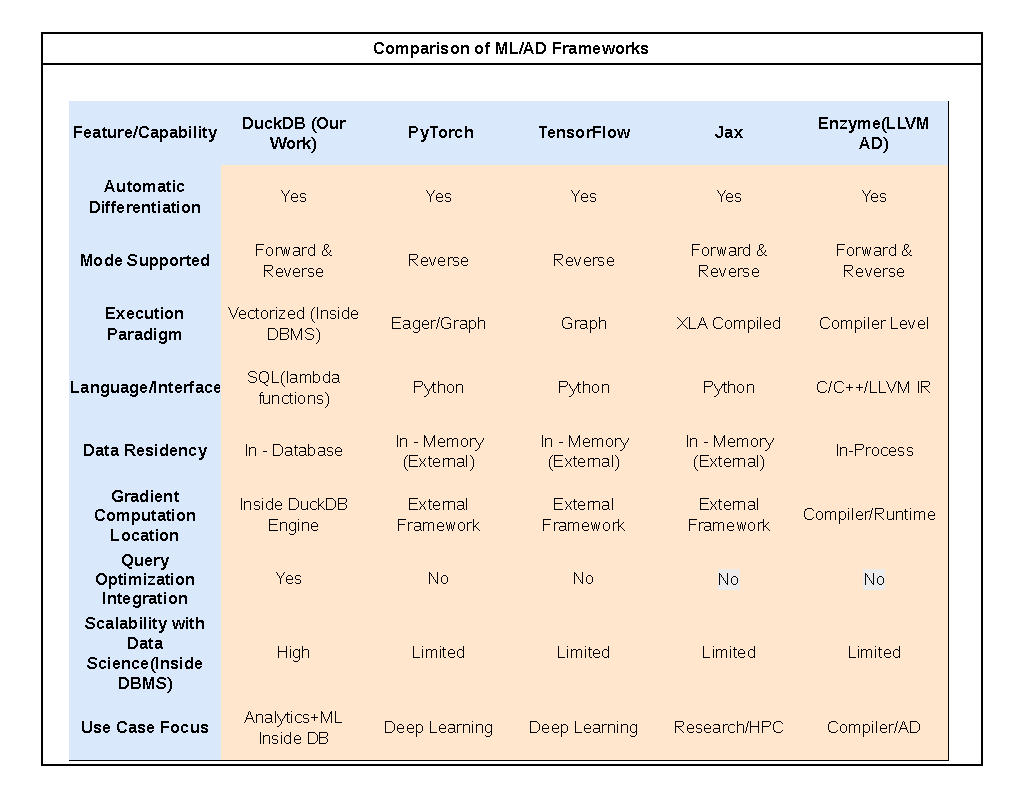
\includegraphics[width=\linewidth]{ml_frameworks_comparison.pdf}
\caption{Comparison of automatic differentiation support across DuckDB and modern machine learning frameworks.}
\label{fig:ml_frameworks_comparison}
\end{figure}

\section{Differentiable Programming}

Differentiable programming extends AD to general-purpose programming languages. Instead of differentiating only tensor operations, differentiable programming systems attempt to differentiate entire programs, including control flow and data structures.

Recent compiler-based approaches focus on program transformation, graph-level
optimization, the design of intermediate representations, and efficient gradient
compilation~\cite{innes2018adjoint,baudart2021stan}.

These ideas influenced the implementation developed in this thesis, especially the optimization of reverse-mode AD using instruction tapes. The concept of compiling a reusable instruction tape at bind time, rather than rebuilding the computation graph per row, directly reflects tape-based AD compilation strategies. Domain-specific compilers for machine learning, such as TVM~\cite{chen2018tvm}, similarly demonstrate that lowering high-level computations to a compact, optimizable intermediate representation yields substantial runtime benefits.

Most differentiable programming systems, however, focus on tensor programs,
imperative programming languages, or neural-network-oriented computation.

Very little work studies differentiability directly inside SQL query engines or relational algebra execution. A notable exception is the use of differentiable formulations to incorporate relational background knowledge into learning systems~\cite{payani2020relational}, although such work targets logic-based reasoning rather than gradient computation over SQL expressions.

This thesis extends differentiable programming concepts into SQL by enabling gradient computation over higher-order SQL lambda expressions inside DuckDB~\cite{peseux2023differentiable}.

\section{Machine Learning Inside Databases}

There has been significant interest in integrating machine learning functionality directly inside database systems. One major motivation is to avoid unnecessary data movement between storage systems and external machine learning frameworks. Early work even explored embedding neural-network models directly within database systems~\cite{schikuta2008neural}, anticipating the closer coupling of learning and data management seen today.

Early systems include MADlib~\cite{madlib}, which provides SQL-based machine
learning operators for PostgreSQL, and Bismarck~\cite{feng2012unified}, which
introduced a unified architecture for implementing iterative ML and analytical
tasks inside DBMSs.

Large-scale analytical systems such as Spark SQL and MLlib also demonstrated the advantages of combining relational processing with machine learning workloads~\cite{armbrust2015sparksql,zaharia2016spark,meng2016mllib,boehm2016systemml}. These systems build on a broader lineage of large-scale data-processing frameworks, including MapReduce~\cite{dean2004mapreduce}, resilient distributed datasets~\cite{zaharia2012rdd}, declarative dataflow languages such as Pig Latin~\cite{olston2008piglatin}, hybrid MapReduce--DBMS architectures such as HadoopDB~\cite{abouzeid2009hadoopdb}, and interactive web-scale analytical engines such as Dremel~\cite{melnik2010dremel}.

Despite these advances, existing systems typically rely on manually derived
gradients, predefined ML operators, or fixed model templates.

Most systems do not support reusable automatic differentiation directly over arbitrary SQL lambda expressions. The need for automation is reinforced by the difficulty of interpreting and trusting model behaviour, a concern that has motivated dedicated explanation techniques~\cite{ribeiro2016trust}: pipelines whose gradients are derived automatically are easier to inspect and reason about than hand-derived ones.

\begin{figure}[H]
    \centering
    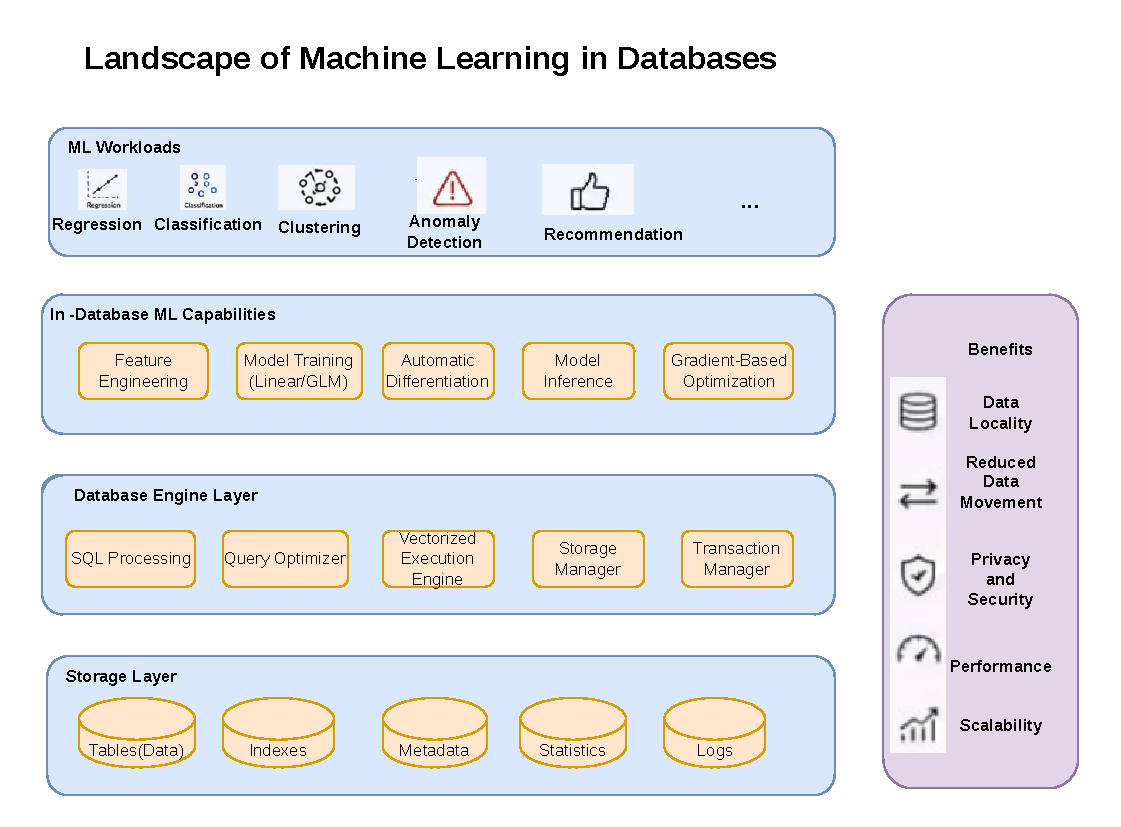
\includegraphics[width=\linewidth]{ml_database_landscape.pdf}
    \caption{Landscape of machine learning approaches integrated inside database systems.}
    \label{fig:ml_landscape}
\end{figure}

The goal of this thesis is different. Instead of implementing predefined ML algorithms, the work focuses on enabling generic automatic differentiation inside DuckDB queries.

\section{Higher-Order Functions in SQL}

Higher-order SQL functions allow functions or lambda expressions to be passed as arguments to other functions. These features increase the expressiveness of SQL and enable a more functional style of query processing.

DuckDB recently introduced support for higher-order functions and lambda expressions. This enables queries such as:

\begin{lstlisting}[language=SQL]
SELECT transform(col, x -> x * 2) FROM t;
\end{lstlisting}

These lambda functions are important for this thesis because they allow mathematical expressions to be represented directly inside SQL queries.

In this work, lambda expressions are treated as differentiable programs. The AD system extracts the lambda expression during query binding and transforms it into an internal representation used for gradient computation.

\begin{figure}[h]
\centering
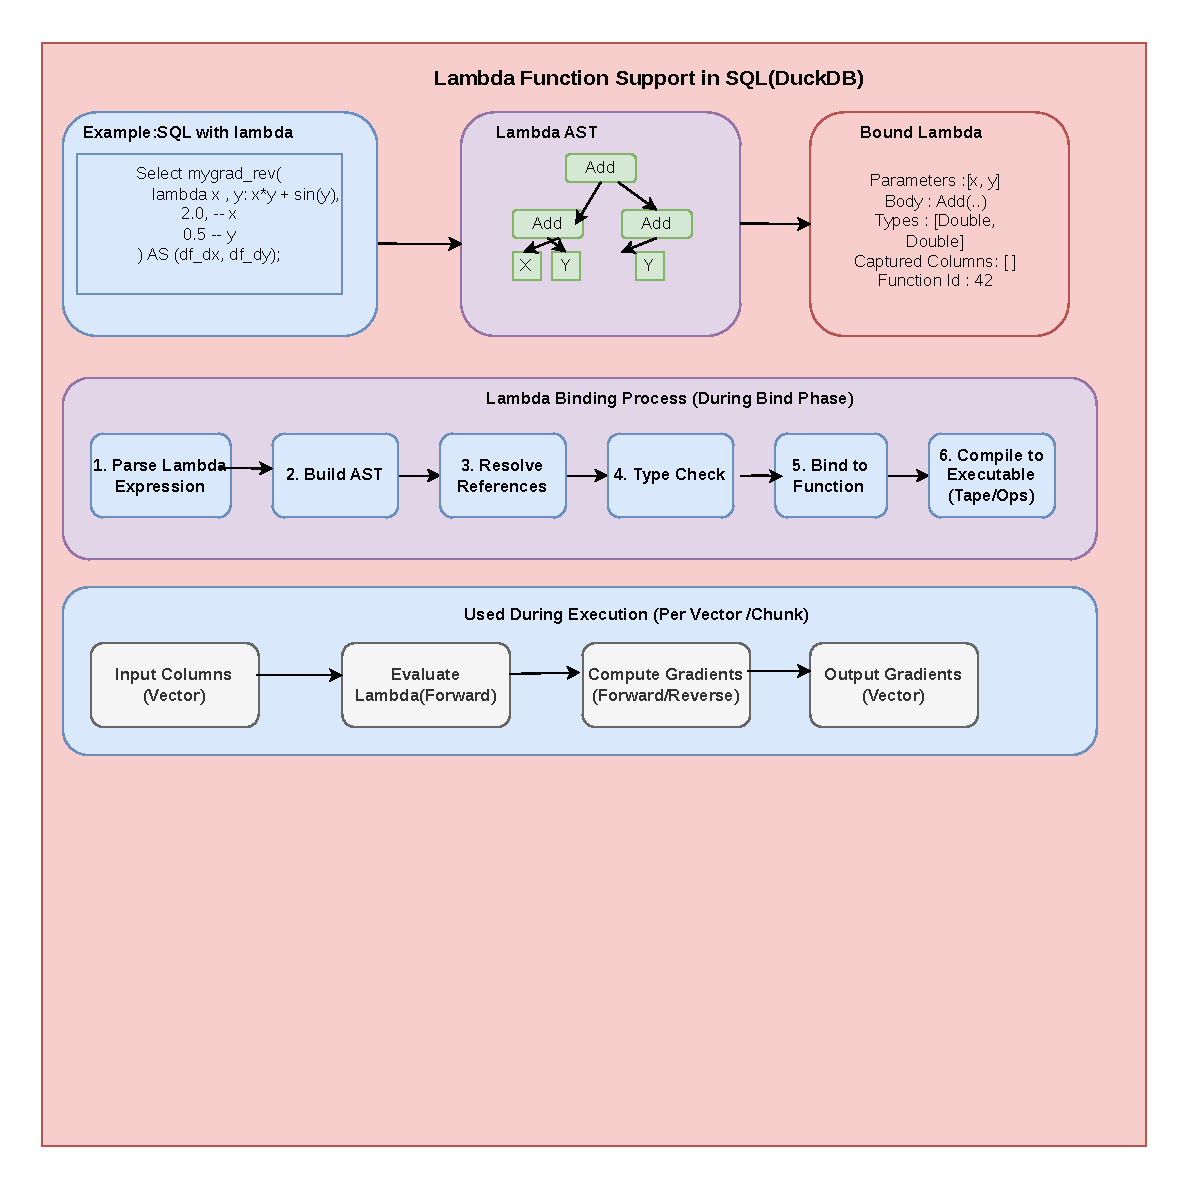
\includegraphics[width=\linewidth]{lambda_support_in_sql.pdf}
\caption{Lambda function support in DuckDB: parsing, binding, and use during execution.}
\label{fig:lambda_support_sql}
\end{figure}

This functionality forms the foundation of the implemented AD framework.

\section{Computation Graphs and AD Execution Models}

Reverse-mode AD relies on computation graphs, also known as tapes, that store intermediate operations and their dependencies during execution. During the backward pass, gradients are propagated in reverse order through the graph.

Deep learning systems such as TensorFlow and PyTorch internally build
computation graphs~\cite{agrawal2019eager} that record primitive operations,
intermediate values, and the dependency relationships required for
backpropagation.

The reverse-mode algorithm itself has a long history. Beyond the deep learning frameworks above, it has been studied both as a functional-programming construct~\cite{pearlmutter2008reverse} and in relation to the underlying error-propagation mechanism of backpropagation~\cite{grum2023backprop}.

DuckDB, however, is not a tensor interpreter. It uses a vectorized query execution engine optimized for columnar analytical processing~\cite{raasveldt2022modular}. Integrating reverse-mode AD into this setting therefore required that lambda expressions be converted into executable operation sequences, that intermediate values be stored efficiently, and that gradients be accumulated within execution chunks.

An early version of the reverse-mode implementation rebuilt the computation graph repeatedly during execution, which produced significant runtime overhead.

To remove this overhead, the computation graph is compiled once, during the bind phase, into an instruction tape representation. The tape stores preprocessed operations that are reused during query execution.

This optimization reduced graph reconstruction overhead and substantially improved reverse-mode runtime.

\begin{figure}[h]
\centering
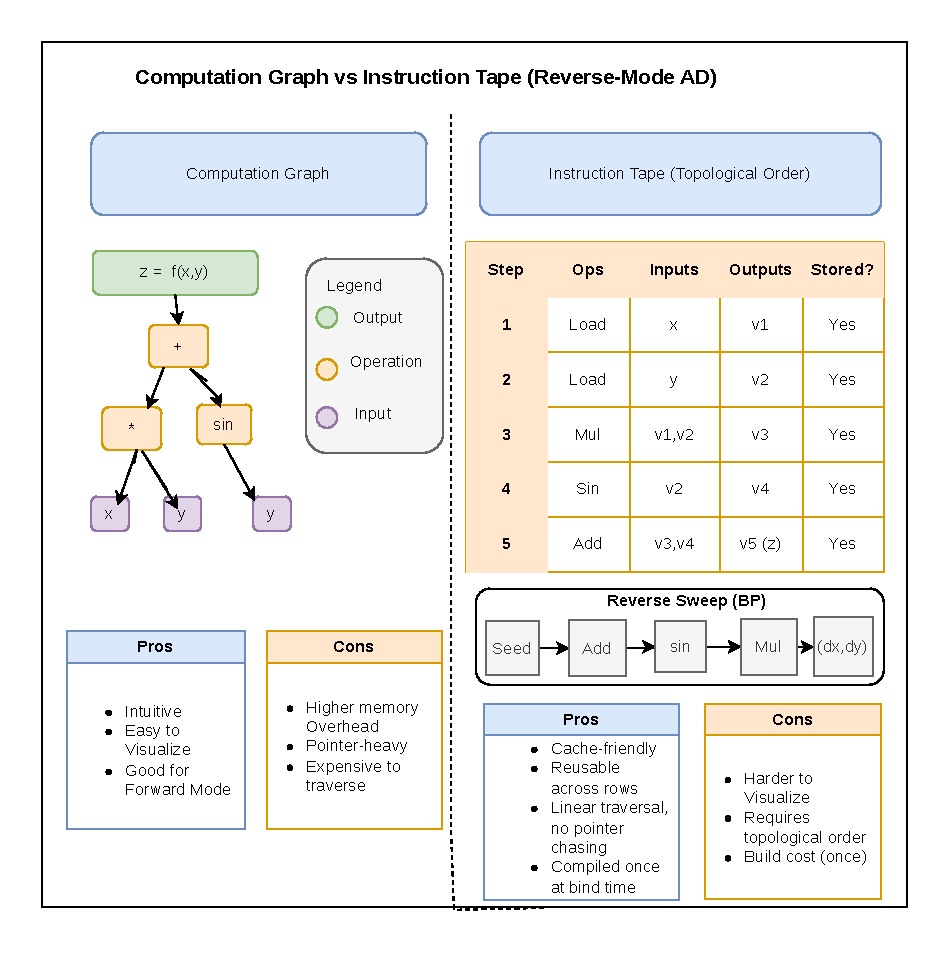
\includegraphics[width=\textwidth]{computation_graph_vs_tape.pdf}
\caption{Comparison between traditional computation graphs and the tape-based reverse-mode implementation used in DuckDB.}
\label{fig:computation_graph_compare}
\end{figure}

This optimization became especially important during the repeated gradient computations in the linear regression benchmarks.

\section{Summary}

This chapter discussed the main background topics required for this thesis, including automatic differentiation, differentiable programming, higher-order SQL functions, and machine learning inside database systems.

Existing systems demonstrate strong interest in combining machine learning and database processing. However, most current approaches rely on predefined operators or external frameworks.

This thesis differs by implementing reusable forward-mode and reverse-mode automatic differentiation directly inside DuckDB using SQL lambda expressions and vectorized query execution.


%%%%%%%%%%%%%%%%%%%%%%%%%%%%%%%%%%%%%%%%%%%%%%%%%%%%
% CHAPTER 3  — DuckDB Architecture & System Design
%%%%%%%%%%%%%%%%%%%%%%%%%%%%%%%%%%%%%%%%%%%%%%%%%%%%

\chapter{DuckDB Architecture and System Design}
\label{ch:design}

DuckDB is a modern in-process analytical database system designed to efficiently execute OLAP-style workloads. Its lightweight architecture, vectorized query execution, and native support for higher-order SQL functions make it an excellent candidate for integrating automatic differentiation (AD). This chapter introduces the primary system components relevant to understanding how AD is integrated into DuckDB.

\section{Overview of DuckDB}

DuckDB differs from traditional client--server databases by running entirely in-process, eliminating network overhead and simplifying integration with analytical tools such as Python and R~\cite{kohn2022duckdbwasm}. It is optimized for OLAP-style analytical workloads, which differ markedly in their access patterns from the transaction-oriented OLTP workloads targeted by main-memory transactional systems such as VoltDB~\cite{stonebraker2013voltdb} and HyPer~\cite{hyper2011}; the contrasting demands of these two workload classes have themselves been the subject of detailed study~\cite{harizopoulos2008oltp}. Its architecture follows a multi-stage query processing pipeline that includes parsing, binding, logical planning, physical planning, and vectorized execution~\cite{raasveldt2022modular}.

Figure~\ref{fig:duckdb_pipeline} illustrates this pipeline.

\begin{figure}[h]
\centering
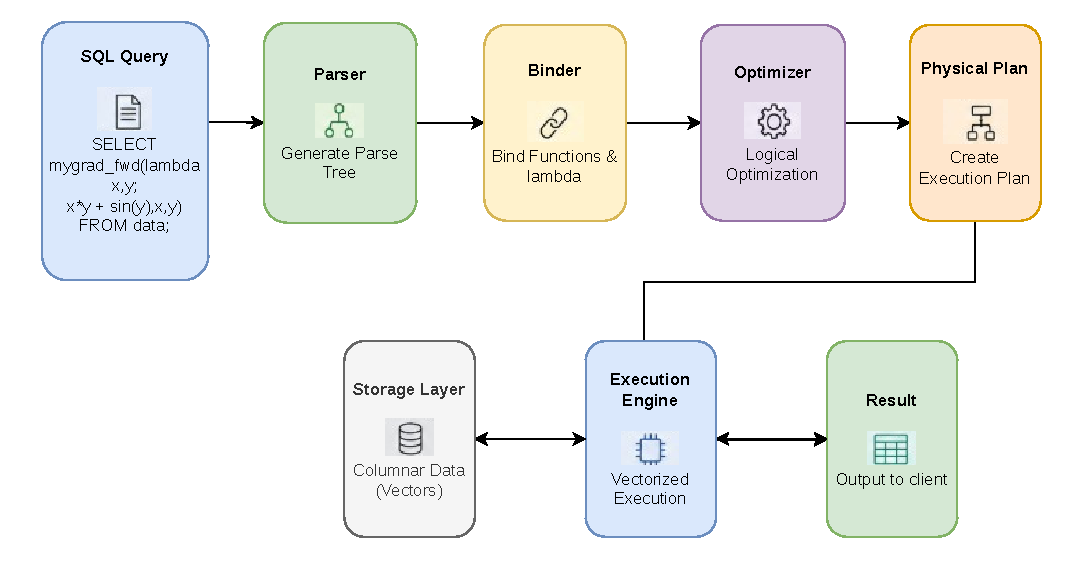
\includegraphics[width=\textwidth]{duckdb_pipeline.pdf}
\caption{DuckDB's query processing pipeline~\cite{duckdb2019,raasveldt2022modular}.}
\label{fig:duckdb_pipeline}
\end{figure}

Each stage plays a distinct role in transforming SQL text into executable operators.

\section{Integration into DuckDB Query Pipeline}

The automatic differentiation framework was integrated into DuckDB's existing query processing pipeline. Instead of modifying the complete execution engine, the implementation extends DuckDB's scalar function subsystem.

The execution flow proceeds in five stages: SQL query parsing, lambda
expression binding, construction of differentiable expressions, forward-mode or reverse-mode AD execution, and finally vectorized result generation. The
implementation reuses DuckDB's vectorized execution engine and operates
directly on \texttt{DataChunk} structures during query execution.

\section{Parsing and Lambda Expressions}

DuckDB supports higher-order SQL functions and lambda expressions, enabling functional programming constructs inside SQL. A lambda such as:

\begin{lstlisting}[language=SQL]
(x -> x + 1)
\end{lstlisting}

\ldots is parsed into a \texttt{LambdaExpression} AST node that stores a list of
parameters, a body expression, and any captured variables. These abstract
syntax trees form the structural representation required by AD.
Figure~\ref{fig:lambda_ast} shows a simplified representation of the lambda
AST.

\begin{figure}[h]
\centering
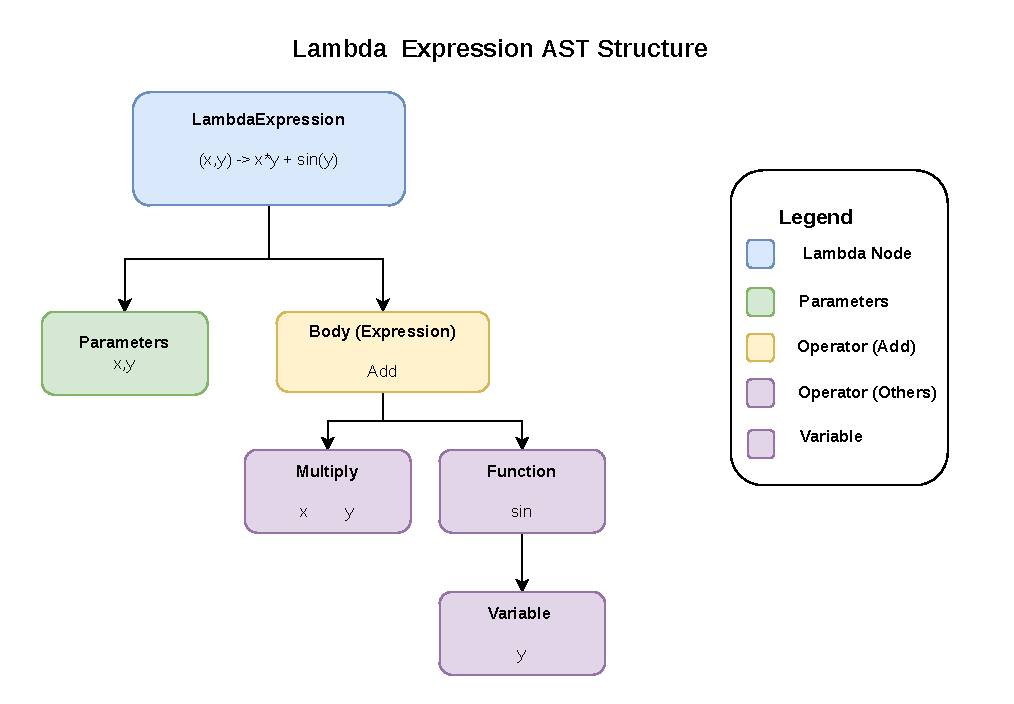
\includegraphics[width=\textwidth]{lambda_ast.pdf}
\caption{Simplified lambda expression AST structure.}
\label{fig:lambda_ast}
\end{figure}

\subsection{Lambda Parameter Binding}

During implementation, lambda expressions required explicit parameter resolution during the binding phase. DuckDB internally represents lambda references using bound expressions, but parameter references were not always consistently mapped across different expression types.

To resolve this, a helper mechanism named \texttt{NameToSlot()} was introduced. The function maps lambda parameter names to the internal parameter indices used during derivative seeding:

\begin{lstlisting}[language=C++]
static bool NameToSlot(
    const string &raw_in,
    idx_t param_cnt,
    idx_t &slot_out);
\end{lstlisting}

This mapping allowed automatic differentiation to correctly associate each lambda parameter with its corresponding derivative vector entry.

\section{Binder: Central Integration Point for AD}

The binder performs semantic analysis, resolves identifiers, infers types, rewrites expressions, and ensures SQL validity. It is also the earliest stage at which a complete expression tree is available. Reverse-mode AD requires constructing a computation graph, or tape, that captures the order of operations~\cite{griewank2008evaluating,baydin2017automatic}. Because binding happens once per query rather than once per row, it is the ideal place to compile this graph.

The AD extension adds binder logic that extracts the expression tree from a
lambda, traverses it once, and builds a reusable computation tape for
reverse-mode AD.

Performing this work in the binder is necessary because lambda references are not always bound consistently across different expression types inside DuckDB, and the binder is the first stage at which the complete, resolved expression tree can be inspected. Shifting work from the per-row execution path to a single binding-time step mirrors the design philosophy of query compilers, which similarly specialize a query before execution to avoid repeated interpretation overhead~\cite{shaikhha2016compiler,tahboub2018compiler}.

Figure~\ref{fig:binder_workflow} shows the binder workflow.

\begin{figure}[h]
\centering
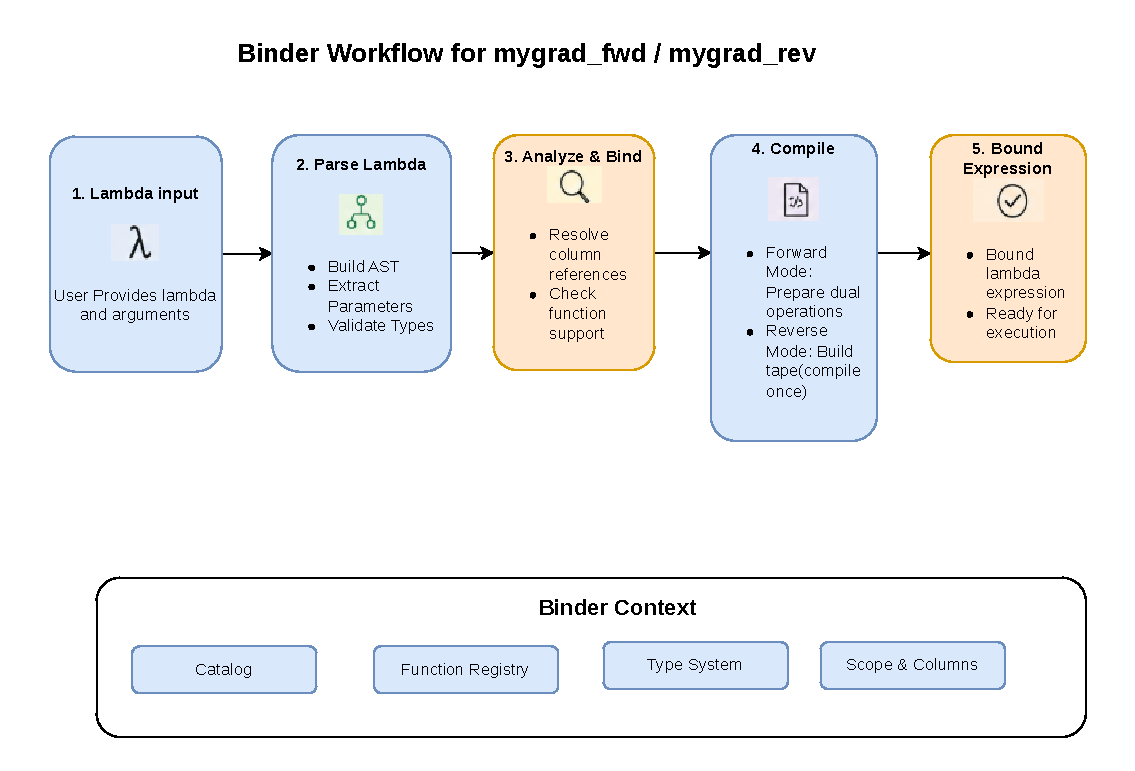
\includegraphics[width=\textwidth]{binder_workflow.pdf}
\caption{Extended binder workflow with reverse-mode AD tape compilation~\cite{griewank2008evaluating}.}
\label{fig:binder_workflow}
\end{figure}

Compiling the tape in the binder significantly improves execution performance, because the tape is then reused for every input row instead of being rebuilt.

\section{Logical and Physical Planning}

After binding, DuckDB builds a logical plan composed of operators such as:

\begin{itemize}
    \item \texttt{LogicalGet} (table scan),
    \item \texttt{LogicalProjection},
    \item \texttt{LogicalFilter},
    \item \texttt{LogicalAggregate}.
\end{itemize}

This planning model is related to classical relational query optimization and execution techniques~\cite{selinger1979access,graefe1993query,neumann2011efficiently,chaudhuri1998optimization,graefe1994volcano}. The interaction between query plans and application code has also been studied from the opposite direction, by synthesizing relational queries from imperative programs~\cite{cheung2013synthesis}, which underscores how closely program structure and query structure are related.

AD-based lambda expressions appear as scalar functions inside projections. The physical planner converts the logical plan into vectorized physical operators~\cite{raasveldt2022modular}, and the AD functions \texttt{mygrad\_fwd} and \texttt{mygrad\_rev} execute inside the \texttt{PhysicalExpressionExecutor}.

\section{Vectorized Execution}

DuckDB's vectorized execution model evaluates operators on \texttt{DataChunk} structures, which typically contain up to 2048 values per column. Each chunk consists of column vectors that are processed efficiently using SIMD-style optimizations~\cite{raasveldt2022modular,kersten2018vectorized,boncz2008monetdb}. This columnar, chunk-at-a-time execution style builds on a long line of work on column-oriented and main-memory database systems~\cite{stonebraker2005cstore,abadi2006compression,harizopoulos2006readoptimized,manegold2002mainmemory}, including strategies for efficiently merging differential update stores into column-oriented in-memory engines~\cite{hubner2011differential}, and on NUMA-aware parallel query evaluation~\cite{leis2014morsel}.

Figure~\ref{fig:vectorized_execution} shows this model.

\begin{figure}[h]
\centering
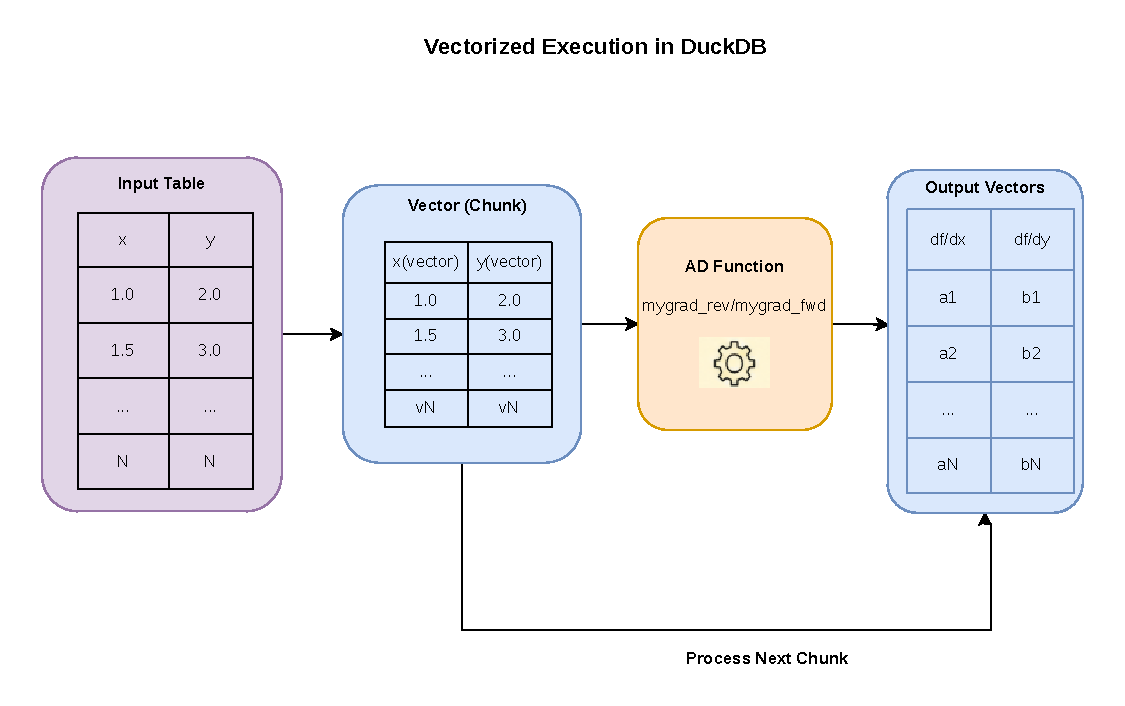
\includegraphics[width=\textwidth]{vectorized_execution.pdf}
\caption{Vectorized execution model used in DuckDB~\cite{raasveldt2022modular}.}
\label{fig:vectorized_execution}
\end{figure}

The AD system integrates into this model at the scalar-function level. The AD functions are invoked once per data chunk: forward-mode AD propagates derivative information alongside the primal values, and reverse-mode AD executes a primal pass followed by adjoint propagation over the compiled tape. Within a chunk, the compiled tape is replayed for each row; the performance implications of this are discussed in Chapter~\ref{ch:conclusion}.

\section{Full AD Integration Across DuckDB}

Figure~\ref{fig:system_architecture} presents the overall system architecture,
which integrates DuckDB's binder and planner, the AD extension layer,
forward-mode and reverse-mode AD, and vectorized runtime execution. This
architecture allows differentiable SQL expressions to be evaluated using
DuckDB's native execution pipeline.

\begin{figure}[h]
\centering
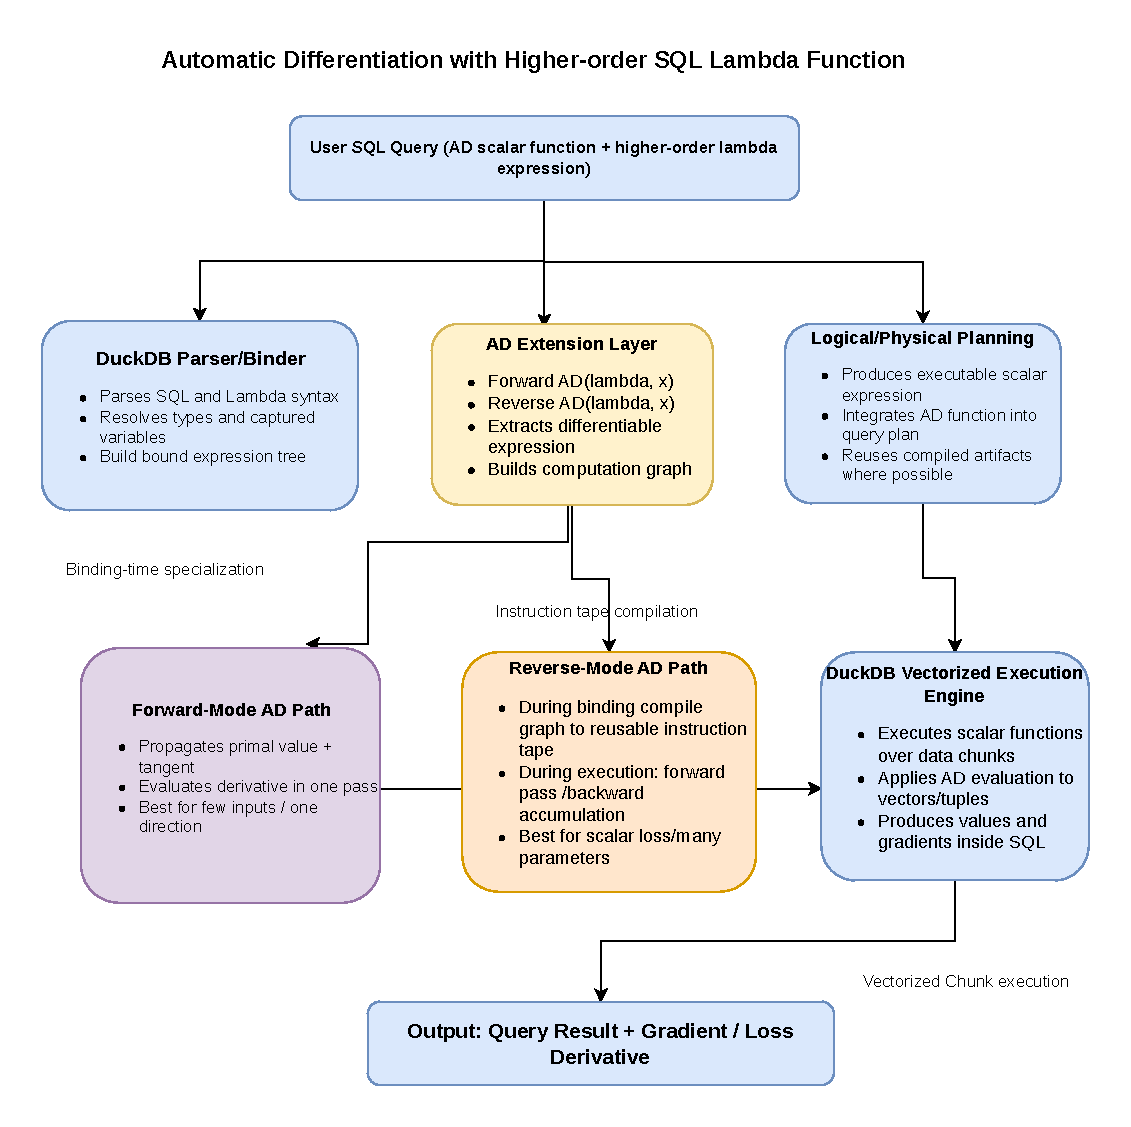
\includegraphics[width=\textwidth]{system_architecture.pdf}
\caption{Overall architecture of the AD extension in DuckDB, integrating forward-mode and reverse-mode AD with higher-order SQL functions~\cite{raasveldt2022modular,baydin2017automatic}.}
\label{fig:system_architecture}
\end{figure}

\section{Summary}

This chapter described DuckDB's architecture and its relevance to integrating AD functionality. The binder provides the crucial entry point for extracting expression trees and compiling reverse-mode AD tapes. The logical and physical planning stages incorporate AD into the execution plan, while DuckDB's vectorized execution engine evaluates both primal values and gradients. During implementation, understanding the binder stage was particularly important, because this is where the lambda expression tree becomes accessible for tape compilation. Chapter~\ref{ch:evaluation} evaluates the performance of these AD mechanisms through empirical experiments.

%%%%%%%%%%%%%%%%%%%%%%%%%%%%%%%%%%%%%%%%%%%%%%%%%%%%
% CHAPTER 4 — Implementation
%%%%%%%%%%%%%%%%%%%%%%%%%%%%%%%%%%%%%%%%%%%%%%%%%%%%

\chapter{Implementation}
\label{ch:implementation}

\section{Overview}

This chapter describes the implementation of automatic differentiation (AD) inside DuckDB using higher-order SQL lambda functions. The goal of the implementation was to support gradient computation directly within SQL queries without relying on external machine learning frameworks.

The implementation was developed directly inside the DuckDB source tree in C++. The AD functionality was integrated into DuckDB's scalar function framework and reused the existing parser, binder, and vectorized execution engine provided by DuckDB~\cite{duckdb2019}.

Two differentiation approaches were implemented:

\begin{itemize}
     \item Forward-mode AD
     \item Reverse-mode AD
\end{itemize}

Both approaches operate on lambda expressions written directly in SQL queries, and both return the full gradient of the lambda expression in a single call.

\section{Implementation Environment}

The implementation was developed on Ubuntu Linux. Two build configurations of DuckDB were used. A debug build with assertions and the address sanitizer enabled was used during development to detect memory and correctness errors, while an optimized release build was used to obtain the performance measurements reported in Chapter~\ref{ch:evaluation}. The following tools were used during development:

\begin{itemize}
    \item DuckDB source code
    \item CMake build system
    \item Ninja build tool
    \item Gnuplot and PGFplots for visualization
    \item Git and GitHub for version control
\end{itemize}

The project repository containing the implementation and benchmark scripts is available at:

\begin{center}
\url{https://github.com/Lechulakshmi821/duckdb-thesis}
\end{center}

\section{Modified Source Files}

The implementation required modifications and additions to several DuckDB source files, together with a set of benchmark scripts.

\begin{table}[H]
\centering
\begin{tabular}{|l|l|}
\hline
File & Purpose \\
\hline
autodiff\_grad.cpp & Forward-mode AD implementation \\
autodiff\_reverse.cpp & Reverse-mode AD implementation \\
duckdb\_func\_generic.cpp & Function registration \\
bench\_baseline.sql.in & Handwritten SQL baseline benchmark \\
bench\_fwd\_single\_call.sql.in & Forward-mode AD benchmark \\
bench\_rev\_single\_call.sql.in & Reverse-mode AD benchmark \\
run\_compare\_bench\_release.sh & Benchmark automation script \\
aggregate.py & Aggregates raw runs into a median summary \\
\hline
\end{tabular}
\caption{Main implementation and benchmark files}
\label{tab:impl-files}
\end{table}

\section{Forward-Mode Automatic Differentiation}

Forward-mode AD propagates derivative information alongside primal values during expression evaluation. Conceptually, each value is extended into a dual number:

\begin{equation}
(v, \dot{v})
\label{eq:dual-number}
\end{equation}

where \(v\) is the original value and \(\dot{v}\) is its derivative.

In the implemented design, a single scalar derivative is generalised to a vector of partial derivatives, so that the partials with respect to all lambda parameters can be propagated in one evaluation pass. Each intermediate value therefore stores the computed scalar value together with a gradient vector. This is represented by the following structure:

\begin{lstlisting}[language=C++]
struct Dual {
    double val;
    std::vector<double> grad;
};
\end{lstlisting}

Arithmetic operators for addition, subtraction, multiplication, and division were overloaded to propagate derivatives according to the chain rule. Because the gradient vector carries one entry per parameter, the cost of forward-mode evaluation grows with the number of parameters; this property is analysed further in Appendix~\ref{app:proofs} and is reflected in the experimental results in Chapter~\ref{ch:evaluation}.


\section{Bind-Time Operator Resolution}

An early version of the forward-mode evaluator dispatched arithmetic
operators by performing string operations on every operator in every
row: \texttt{StringUtil::Lower(ExpressionTypeToString(expr.type))} followed
by several substring searches to determine whether the operator was
ADD, SUB, MUL, or DIV. For an expression of approximately 50 operators
evaluated over 50{,}000 rows for 20 gradient-descent iterations, this
amounted to tens of millions of string operations per benchmark run
and dominated the forward-mode runtime.

The optimized design moves this work to the bind phase. During binding,
the expression tree is walked once and each operator's kind is resolved
into a compact \texttt{OpKind} enum, cached in a hash map keyed by the
expression pointer:

\begin{lstlisting}[language=C++]
enum class OpKind { ADD, SUB, MUL, DIV, NEG, UNKNOWN };

struct AutoDiffGradBindData : public FunctionData {
    unique_ptr<Expression> lambda_expr;
    idx_t param_cnt;
    std::unordered_map<Expression*, OpKind> op_cache;
    // ...
};
\end{lstlisting}

At execution time, \texttt{EvalExpr} performs a single hash-map lookup
followed by a \texttt{switch} statement on the enum, with no per-row
string operations:

\begin{lstlisting}[language=C++]
auto it = bind.op_cache.find(&expr);
OpKind kind = (it != bind.op_cache.end())
              ? it->second : OpKind::UNKNOWN;

switch (kind) {
case OpKind::ADD: return Add(L, R);
case OpKind::SUB: return Sub(L, R);
case OpKind::MUL: return Mul(L, R);
case OpKind::DIV: return Div(L, R);
case OpKind::NEG: return Neg(L);
default:
    throw BinderException("mygrad: unsupported operator");
}
\end{lstlisting}

This mirrors the design philosophy of the reverse-mode AD's compiled
instruction tape: expensive analysis is performed once at bind time
and replayed cheaply per row. The effect of this optimization on
runtime is reported in Chapter~\ref{ch:evaluation}.

\section{Expression Evaluation}

DuckDB internally represents SQL expressions as expression trees. The implementation recursively traverses these expression trees and propagates derivative information through the computation.

The following expression types are supported:

\begin{itemize}
    \item Constants
    \item Column references
    \item Arithmetic operators
    \item Unary negation
    \item Cast expressions
\end{itemize}

Unsupported expressions raise runtime exceptions during query execution.

\section{Lambda Function Integration}

Higher-order lambda functions are used to represent differentiable computations directly inside SQL queries. The AD function receives a list of numeric arguments followed by a lambda expression. The lambda declares one parameter per numeric argument, in the same positional order, and its body may refer only to those declared parameters. The AD function returns a structured value holding one partial derivative per argument; the gradient with respect to the trainable parameters is read from the corresponding struct fields.

An example forward-mode query is shown below:

\begin{lstlisting}[language=SQL]
SELECT mygrad_fwd(
    a1, a2, x1, y,
    (p1, p2, p3, p4) ->
        (p1 * p3 + p2 - p4) * (p1 * p3 + p2 - p4)
)
FROM data;
\end{lstlisting}

For readability, the example above uses a simplified four-parameter lambda expression. The actual benchmark workload described in Chapter~\ref{ch:evaluation} uses six trainable weights and one bias parameter.

During binding, the lambda expression is extracted from the function arguments and stored in internal bind data structures for use during execution.

\section{Parameter Mapping}

One implementation challenge involved mapping lambda parameter names to gradient slots.

In some cases, DuckDB represented lambda variables as generic bound references rather than positional parameters. To resolve this, a name-based mapping helper was implemented:

\begin{lstlisting}[language=C++]
static bool NameToSlot(const string &raw_in,
                       idx_t param_cnt,
                       idx_t &slot_out);
\end{lstlisting}

This function maps lambda parameter names such as \texttt{p1}, \texttt{p2}, or \texttt{p3} to the corresponding gradient index used during derivative seeding.

\section{Reverse-Mode Automatic Differentiation}

Reverse-mode AD was implemented using a compiled instruction tape and backward propagation~\cite{baydin2017automatic}.

Rather than interpreting the lambda expression tree directly, the expression is compiled into a flat sequence of primitive operations. Each operation is represented by a compact record storing the operation kind and the indices of its operand operations:

\begin{lstlisting}[language=C++]
struct CompiledOp {
    OpKind  op;          // INPUT, CONST, NEG, ADD, SUB, MUL, DIV
    int32_t a, b;        // operand indices into the program
    double  cval;        // constant value (CONST only)
    int32_t input_slot;  // parameter slot (INPUT only)
};
\end{lstlisting}

The compiled program is a single \texttt{std::vector<CompiledOp>}, which is contiguous in memory and indexed by integer position rather than traversed through pointers. Evaluation proceeds in two phases. During the forward pass, the operations are evaluated in order and their primal values stored. During the backward pass, the program is traversed in reverse, and adjoint values are accumulated into each operand according to the local derivative rule of each operation.

\subsection{Bind-Time Tape Compilation and Reuse}

An early version of the reverse-mode implementation reconstructed the computation graph during query execution. Because the same lambda expression structure was analysed repeatedly, this introduced significant overhead for larger datasets.

To remove this overhead, the expression tree is compiled into the instruction tape exactly once, during the binding phase. Binding occurs once per query rather than once per row, so the compiled tape is produced a single time and stored in the function's bind data. During execution the tape is only read; it is not rebuilt. The tape is therefore shared across every gradient-descent iteration and every processed row.

This optimization eliminates repeated graph construction and is the most important performance improvement implemented in this work. Its effect is discussed in Chapter~\ref{ch:evaluation} and Appendix~\ref{app:experiments}.

\section{Reverse-Mode Execution Workflow}

The overall reverse-mode workflow separates the one-time tape compilation in the binder from the per-row replay in the execution engine, as shown in Algorithm~\ref{alg:reverse-ad}.

\begin{algorithm}
\caption{Reverse-Mode AD with Bind-Time Tape Reuse}
\label{alg:reverse-ad}
\begin{algorithmic}
\State \textbf{Bind phase (once per query):}
\State \quad Parse and bind the lambda expression
\State \quad Compile the expression tree into an instruction tape
\State \quad Store the compiled tape in the function bind data
\State \textbf{Execution phase (per data chunk):}
\State \quad Allocate primal and adjoint buffers once for the chunk
\ForAll{rows in the chunk}
    \State Reset the adjoint buffer
    \State Execute the forward pass over the tape, storing primal values
    \State Seed the adjoint of the output operation with $1.0$
    \State Execute the backward pass over the tape, accumulating adjoints
    \State Emit the parameter gradients for the row
\EndFor
\end{algorithmic}
\end{algorithm}

\section{Modified DuckDB Components}

The implementation required modifications to the following DuckDB source files:

\begin{itemize}
    \item \texttt{src/function/scalar/generic/autodiff\_grad.cpp}
    \item \texttt{src/function/scalar/generic/autodiff\_reverse.cpp}
    \item \texttt{src/function/scalar/generic/duckdb\_func\_generic.cpp}
\end{itemize}

The AD functions were integrated into DuckDB's scalar function framework and registered using \texttt{ScalarFunctionSet}.

\subsection{Function Registration}

The forward-mode and reverse-mode functions were registered under separate names:

\begin{lstlisting}[language=C++]
ScalarFunctionSet fwd_set("mygrad_fwd");
ScalarFunctionSet rev_set("mygrad_rev");
\end{lstlisting}

Initially, benchmark queries referenced the name \texttt{mygrad}, which did not correspond to any registered function and caused catalog errors during execution. The benchmark scripts were updated to use the registered names \texttt{mygrad\_fwd} and \texttt{mygrad\_rev} explicitly.

\section{Integration with Vectorized Execution}

DuckDB executes queries using vectorized processing~\cite{duckdb2019}. Instead of processing one tuple at a time, the engine evaluates operators over chunks of tuples.

The AD implementation integrates with this model at the scalar-function level. For each data chunk, the execution function reads the compiled tape from the bind data and allocates the primal and adjoint buffers once. It then replays the tape for each row in the chunk, writing the resulting gradients into the output vector. Allocating the working buffers per chunk rather than per row avoids repeated memory allocation in the evaluation loop.

This design allowed the implementation to integrate naturally with the existing execution pipeline while avoiding major changes to DuckDB internals. It should be noted that the tape itself is replayed one row at a time; the AD operations are not vectorized across the chunk. The performance implications of this are discussed in Chapter~\ref{ch:conclusion}.

\section{Implementation Challenges}

Several implementation issues were encountered during development.

\subsection{Duplicate Symbol Errors}

During compilation, the forward-mode and reverse-mode implementations initially used identical internal structure and function names. Because DuckDB uses unity builds, which concatenate multiple source files into a single translation unit, this caused duplicate-definition errors such as:

\begin{lstlisting}
redefinition of 'struct AutoDiffGradBindData'
redefinition of 'struct RowInput'
\end{lstlisting}

The issue was resolved by giving the reverse-mode implementation distinct internal structure names and registration functions, separate from those used in the forward-mode implementation.

\section{Summary}

This chapter described the implementation of automatic differentiation inside DuckDB using higher-order SQL lambda functions. Forward-mode AD was implemented through dual-number propagation, while reverse-mode AD was implemented as an instruction tape compiled once at bind time and replayed during vectorized execution. Both modes return the full gradient in a single call and were integrated into DuckDB's scalar function framework, reusing the existing parser, binder, and execution engine.

Several implementation challenges were addressed during development, including lambda parameter binding, function registration conflicts, and duplicate-symbol errors arising from unity builds. The final implementation successfully supported automatic gradient computation directly inside SQL queries.

%%%%%%%%%%%%%%%%%%%%%%%%%%%%%%%%%%%%%%%%%%%%%%%%%%%%
% CHAPTER 5 — Experimental evaluation
%%%%%%%%%%%%%%%%%%%%%%%%%%%%%%%%%%%%%%%%%%%%%%%%%%%%

\chapter{Experimental Evaluation}
\label{ch:evaluation}

\section{Overview}

This chapter evaluates the performance of the proposed automatic differentiation framework implemented in DuckDB. The experiments compare handwritten SQL gradients, forward-mode automatic differentiation, and reverse-mode automatic differentiation on linear regression workloads. Linear regression was chosen because analytical gradients are known, allowing direct correctness verification.

The main goal of the evaluation is to study the runtime overhead of automatic
differentiation inside SQL, its scalability with increasing tuple counts, the
performance difference between forward-mode and reverse-mode AD, and the effect of instruction tape reuse in reverse-mode AD.

All experiments were executed directly inside DuckDB without external machine learning frameworks.

\section{Experimental Setup}

The experiments were conducted on a local Linux environment. The AD implementation was integrated into DuckDB as scalar functions.

All performance measurements reported in this chapter were obtained using an optimized release build of DuckDB, compiled with the \texttt{-O3} optimization level. A separate debug build with assertions and the address sanitizer enabled was used during development for correctness checking, but was not used for performance measurement, since sanitizer instrumentation inflates absolute runtimes by a large and method-dependent factor.

The benchmark environment consists of:

\begin{itemize}
    \item DuckDB optimized release build with AD extensions
    \item Ubuntu Linux environment
    \item C++ implementation integrated into the DuckDB source code
    \item SQL benchmark scripts executed through the DuckDB CLI
\end{itemize}

The benchmark was driven by the following scripts:

\begin{itemize}
    \item \texttt{bench\_baseline.sql.in}
    \item \texttt{bench\_fwd\_single\_call.sql.in}
    \item \texttt{bench\_rev\_single\_call.sql.in}
    \item \texttt{run\_compare\_bench\_release.sh}
    \item \texttt{aggregate.py}
\end{itemize}

\section{Benchmark Workload}

The benchmark uses linear regression with squared loss. Synthetic datasets were generated directly inside DuckDB using random floating-point values.

The benchmark computes the following loss function:

\begin{equation}
L = (\mathit{prediction} - y)^2
\end{equation}

where:

\begin{equation}
\mathit{prediction} = a_1x_1 + a_2x_2 + a_3x_3 + a_4x_4 + a_5x_5 + a_6x_6 + b
\end{equation}

The workload uses six input features, six trainable weights, and a single bias
parameter, with squared loss and twenty gradient-descent iterations.

The dataset sizes evaluated were 1{,}000, 5{,}000, 10{,}000, 20{,}000, and 50{,}000 tuples.

Each configuration was executed five times. The median runtime is reported, and the minimum and maximum runtimes were also recorded to assess measurement stability.

\section{Compared Methods}

Three implementations were evaluated.

\subsection{Handwritten SQL Baseline}

The baseline implementation manually computes the analytical gradients directly in SQL using handwritten arithmetic expressions. This approach represents a hand-tuned SQL implementation, since the gradients are pre-derived by hand and no automatic differentiation machinery is involved during execution.

\subsection{Forward-Mode Automatic Differentiation}

Forward-mode AD propagates derivatives during expression evaluation using the chain rule. Each value carries both the original numeric value and a gradient vector containing one partial derivative per parameter. The implementation is exposed as the scalar function \texttt{mygrad\_fwd}.

\subsection{Reverse-Mode Automatic Differentiation}

Reverse-mode AD is implemented using a compiled instruction tape. During binding, the lambda expression is compiled once into a reusable sequence of primitive operations. The implementation is exposed as the scalar function \texttt{mygrad\_rev}.

Execution performs a forward evaluation pass followed by a reverse adjoint propagation pass. Unlike an earlier version of the implementation, the optimized version reuses the compiled instruction tape across all rows instead of rebuilding the computation graph for every row.

\section{Benchmark Script}

The benchmark execution was automated using a shell script that iterates over the dataset sizes and the three methods, repeating each measurement five times. The following fragment shows the timed execution:

\begin{lstlisting}[language=bash]
   DUCKDB_BIN="./build/release/duckdb"
   SIZES=(1000 5000 10000 20000 50000)
   REPEAT=5
   
   for n in "${SIZES[@]}"; do
     for r in $(seq 1 "${REPEAT}"); do
       sed "s/__N__/${n}/g" "${SQL_FILE}" > "${SQL_TMP}"
       /usr/bin/time -f "%e" -o "${TIME_TMP}" \
           "${DUCKDB_BIN}" < "${SQL_TMP}" > /dev/null
       echo "${n},${METHOD},${r},$(cat "${TIME_TMP}")" \
           >> "${OUTCSV}"
     done
   done
\end{lstlisting}

Each method is benchmarked by a separate SQL script, so that the measured wall-clock time of one method never includes the cost of another. Every individual run is recorded to a raw CSV file, with one row per dataset size, method, and repetition. A separate aggregation step then computes the median per configuration and writes a summary CSV, which is used directly as the input table for the plotting tool.

\section{Scalability Results}

Table~\ref{tab:runtime-results} shows the median runtime for all evaluated methods on the optimized release build.

\begin{table}[H]
\centering
\begin{tabular}{|c|c|c|c|}
\hline
Tuples & Baseline (s) & Forward AD (s) & Reverse AD (s) \\
\hline
1,000  & 0.03 & 0.06 & 0.04 \\
5,000  & 0.05 & 0.21 & 0.05 \\
10,000 & 0.04 & 0.32 & 0.07 \\
20,000 & 0.06 & 0.70 & 0.13 \\
50,000 & 0.11 & 1.47 & 0.24 \\
\hline
\end{tabular}
\caption{Median runtime comparison of baseline SQL, forward-mode AD, and reverse-mode AD (optimized release build, median of five runs, single-threaded with \texttt{PRAGMA threads=1}).}
\label{tab:runtime-results}
\end{table}

\begin{figure}[H]
\centering
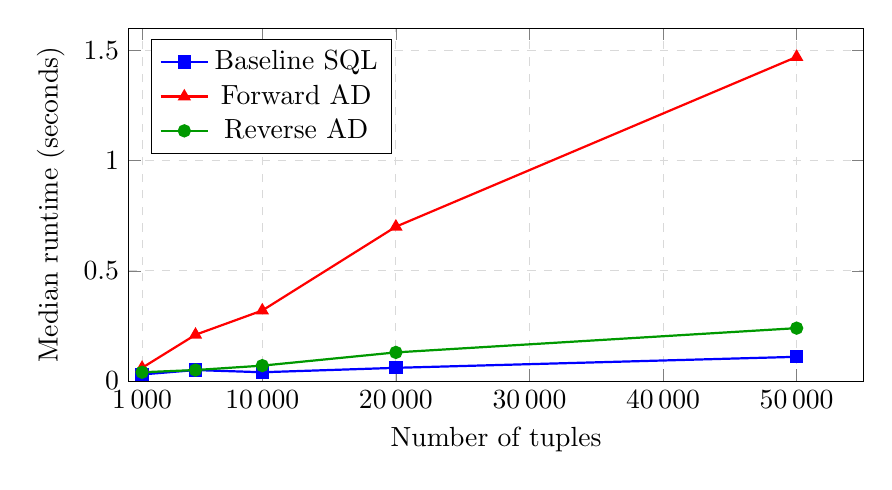
\begin{tikzpicture}
\begin{axis}[
    width=0.9\textwidth,
    height=0.5\textwidth,
    xlabel={Number of tuples},
    ylabel={Median runtime (seconds)},
    xmin=0, xmax=55000,
    ymin=0, ymax=1.6,
    xtick={1000,10000,20000,30000,40000,50000},
    scaled x ticks=false,
    xticklabel style={/pgf/number format/1000 sep=\,},
    legend pos=north west,
    grid=major,
    grid style={dashed,gray!30},
]

\addplot[color=blue, mark=square*, thick] coordinates {
    (1000, 0.03)
    (5000, 0.05)
    (10000, 0.04)
    (20000, 0.06)
    (50000, 0.11)
};
\addlegendentry{Baseline SQL}

\addplot[color=red, mark=triangle*, thick] coordinates {
    (1000, 0.06)
    (5000, 0.21)
    (10000, 0.32)
    (20000, 0.70)
    (50000, 1.47)
};
\addlegendentry{Forward AD}

\addplot[color=green!60!black, mark=*, thick] coordinates {
    (1000, 0.04)
    (5000, 0.05)
    (10000, 0.07)
    (20000, 0.13)
    (50000, 0.24)
};
\addlegendentry{Reverse AD}

\end{axis}
\end{tikzpicture}
\caption{Scalability comparison of baseline SQL, forward-mode AD, and reverse-mode AD across different dataset sizes.}
\label{fig:scaling_plot}
\end{figure}


Figure~\ref{fig:runtime-bars} shows the same data as a grouped bar chart, making the gap between forward-mode AD and the other two methods immediately visible.

\begin{figure}[H]
\centering
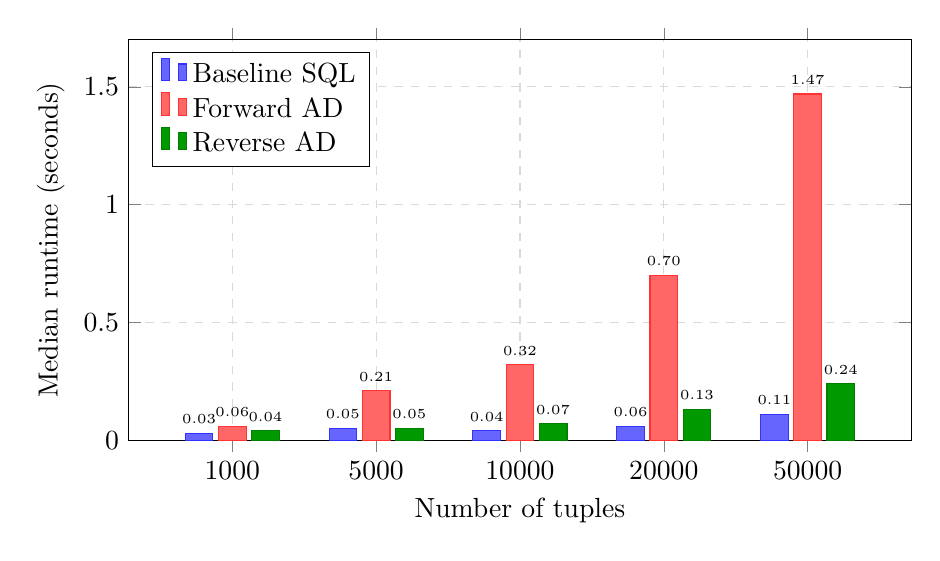
\begin{tikzpicture}
\begin{axis}[
    width=0.95\textwidth,
    height=0.55\textwidth,
    ybar,
    bar width=10pt,
    ymin=0, ymax=1.7,
    ylabel={Median runtime (seconds)},
    symbolic x coords={1000,5000,10000,20000,50000},
    xtick=data,
    xlabel={Number of tuples},
    legend pos=north west,
    legend cell align=left,
    grid=major,
    grid style={dashed,gray!30},
    enlarge x limits=0.18,
    nodes near coords,
    point meta=explicit symbolic,
    every node near coord/.append style={
        font=\tiny,
        rotate=0,
        anchor=south,
    },
]

\addplot[fill=blue!60, draw=blue!80] coordinates {
    (1000, 0.03) [0.03]
    (5000, 0.05) [0.05]
    (10000, 0.04) [0.04]
    (20000, 0.06) [0.06]
    (50000, 0.11) [0.11]
};
\addlegendentry{Baseline SQL}

\addplot[fill=red!60, draw=red!80] coordinates {
    (1000, 0.06) [0.06]
    (5000, 0.21) [0.21]
    (10000, 0.32) [0.32]
    (20000, 0.70) [0.70]
    (50000, 1.47) [1.47]
};
\addlegendentry{Forward AD}

\addplot[fill=green!60!black, draw=green!50!black] coordinates {
    (1000, 0.04) [0.04]
    (5000, 0.05) [0.05]
    (10000, 0.07) [0.07]
    (20000, 0.13) [0.13]
    (50000, 0.24) [0.24]
};
\addlegendentry{Reverse AD}

\end{axis}
\end{tikzpicture}
\caption{Runtime comparison between baseline SQL, forward-mode AD, and reverse-mode AD across different dataset sizes. Values above each bar show the median runtime in seconds.}
\label{fig:runtime-bars}
\end{figure}

\section{Analysis of Results}

The results show that handwritten SQL gradients remain the fastest
approach, because the derivatives are pre-derived by hand and execute
as fused arithmetic expressions that DuckDB's vectorized engine
evaluates efficiently.

Forward-mode AD introduces the highest overhead. Every intermediate
value propagates a complete gradient vector, so the amount of derivative
computation grows with the number of parameters. As the number of
tuples increases, this cost grows accordingly, and forward-mode AD
remains the slowest of the three methods even after the bind-time
operator-resolution optimization described in Chapter~\ref{ch:implementation}.

Reverse-mode AD performs substantially better than forward-mode AD.
The compiled instruction tape is generated once at bind time and reused
for every input row, so the per-row cost is reduced to tape replay
alone. At 50{,}000 tuples, the three methods required approximately:

\begin{itemize}
    \item Baseline SQL: 0.11 seconds
    \item Reverse-mode AD: 0.24 seconds
    \item Forward-mode AD: 1.47 seconds
\end{itemize}

Reverse-mode AD stays close to the handwritten baseline across all
dataset sizes, ranging from roughly $1.3\times$ the baseline runtime
at 1{,}000 tuples to roughly $2.2\times$ at 50{,}000 tuples. This is a
small, near-constant overhead: the AD tape is interpreted operation by
operation and replayed one row at a time, whereas the handwritten
baseline executes as fused arithmetic across whole column vectors, yet
the two remain within the same order of magnitude.

The advantage of reverse-mode AD over forward-mode AD widens with
scale, from roughly $1.5\times$ at 1{,}000 tuples to roughly $6.1\times$
at 50{,}000 tuples. This confirms that reverse-mode cost depends
primarily on the number of operations rather than the number of
parameters: forward-mode AD propagates a gradient vector of length $p$
through every operation, while reverse-mode AD does not. The objective
of the proposed system is not to outperform handwritten SQL gradients
but to compute them automatically; the measured overhead is the modest
price of that automation.

\section{Effect of Instruction Tape Reuse}

An important optimization in the reverse-mode implementation is instruction
tape reuse. A straightforward implementation of reverse-mode AD would
reconstruct the computation graph each time the lambda expression is
evaluated. Because evaluation occurs once per row, this would place graph
construction directly on the per-row execution path. The implemented design
avoids this by exploiting an asymmetry in DuckDB's query pipeline:
\begin{itemize}
    \item The computation graph is compiled into an instruction tape once,
          during the binding phase.
    \item The compiled tape is stored in the function bind data and only
          read during execution.
    \item Only the primal and adjoint values are updated for each row; the
          tape structure itself is never rebuilt.
\end{itemize}
Binding occurs exactly once per query, whereas execution occurs once per row.
Across a workload of $N$ rows and $I$ gradient-descent iterations, compiling
the tape at bind time reduces tape construction from $N \cdot I$ times to a
single time. By construction, this removes repeated graph construction from
the execution path entirely, so the per-row cost is reduced to tape replay
alone. A direct experimental comparison against a per-row-rebuild variant
was outside the scope of this evaluation and is identified as future work;
the benefit of the optimization is argued here from the structure of the
query pipeline rather than measured.

\section{Numerical Correctness Verification}

To verify correctness, the gradients produced by automatic differentiation
were compared against manually derived analytical gradients. For the linear
regression loss, the analytical gradient with respect to a weight is, for
example:

\begin{equation}
\frac{\partial L}{\partial a_1} = 2x_1(\text{prediction} - y)
\end{equation}

The verification was performed over a dataset of 10{,}000 tuples. For every
tuple, all seven gradients (six weights and the bias) produced by both
forward-mode and reverse-mode AD were compared against the corresponding
analytical gradients, and the maximum absolute difference was recorded. For
both AD modes, the maximum difference across all tuples and all parameters was
exactly zero.

This exact agreement is expected. The benchmark loss is a polynomial in the
parameters, so automatic differentiation applies the same sequence of
arithmetic operations (addition, subtraction, and multiplication) as the
analytical gradient expression. Because only exact IEEE-754 operations are
involved, with no transcendental functions or iterative approximations, no
floating-point divergence is introduced. As a sanity check, the same
comparison was repeated against an intentionally perturbed analytical
expression, which produced a clearly non-zero difference; this confirms that
the verification procedure detects discrepancies when they exist. The result
confirms that both the forward-mode and reverse-mode AD implementations are
numerically correct for the evaluated workload.

\section{Implementation Challenges During Benchmarking}

Several issues were encountered during benchmarking.

\subsection{Function Registration Problems}

Initially, the benchmark SQL referenced a function named \texttt{mygrad}, while the forward-mode and reverse-mode implementations were registered separately as \texttt{mygrad\_fwd} and \texttt{mygrad\_rev}. This produced the following error:

\begin{lstlisting}
Catalog Error: Scalar Function with name mygrad does not exist
\end{lstlisting}

The benchmark scripts were updated to use the registered function names explicitly.

\subsection{Duplicate C++ Symbol Definitions}

The forward-mode and reverse-mode implementations initially used identical internal class names, such as \texttt{AutoDiffGradBindData}, \texttt{RowInput}, and \texttt{RegisterAutoDiffGrad}. Because DuckDB uses unity builds, compiling both files together caused redefinition errors. The reverse-mode implementation was renamed to use separate internal structures and registration functions.

\subsection{Isolating the Measured Method}

An earlier version of the benchmark placed the handwritten baseline and an AD method in the same SQL script. As a result, the wall-clock time recorded for the AD method also included the cost of executing the baseline. This was corrected by giving each method its own self-contained script: each script builds the dataset and runs only one method, so the recorded time reflects that method alone.

\subsection{Measurement Variance}

To control measurement variance, each configuration was executed five times and the median runtime was reported. The measurements were generally stable: for most configurations the spread between the minimum and maximum runtime was small. The largest relative variation was observed in two isolated runs, for reverse-mode AD at 5{,}000 and at 50{,}000 tuples, where a single slower run occurred; reporting the median rather than the mean ensures that such outliers do not distort the reported results.

\section{Discussion}

The experiments demonstrate that automatic differentiation can be integrated successfully into DuckDB using higher-order SQL lambda functions. The evaluation shows that:

\begin{itemize}
    \item Forward-mode AD is straightforward to implement but scales poorly as the number of parameters grows.
    \item Reverse-mode AD is consistently faster than forward-mode AD, and its advantage increases with dataset size.
    \item Reverse-mode AD stays within a small, near-constant factor of the handwritten SQL baseline.
    \item Compiling the computation graph once during binding, and reusing it during execution, is the decisive optimization for reverse-mode performance.
\end{itemize}

Although handwritten SQL gradients remain the fastest approach, reverse-mode AD provides greater flexibility, because gradients are derived automatically from a lambda expression rather than written and maintained by hand.

\section{Summary}

This chapter evaluated the performance of the proposed automatic
differentiation framework in DuckDB on an optimized release build,
including the bind-time operator-resolution optimization described in
Chapter~\ref{ch:implementation}. The results show that reverse-mode AD
is consistently faster than forward-mode AD, by a factor that grows
from roughly $1.5\times$ at 1{,}000 tuples to roughly $6.1\times$ at
50{,}000 tuples, while staying within roughly $1.3\times$ to $2.2\times$
of handwritten SQL. The evaluation also confirms that bind-time
compilation --- both for the reverse-mode instruction tape and for the
forward-mode operator cache --- is essential for scalable automatic
differentiation inside a database system.

%%%%%%%%%%%%%%%%%%%%%%%%%%%%%%%%%%%%%%%%%%%%%%%%%%%%
% CHAPTER 6 - Conclusion and Future Work
%%%%%%%%%%%%%%%%%%%%%%%%%%%%%%%%%%%%%%%%%%%%%%%%%%%%

\chapter{Conclusion and Future Work}
\label{ch:conclusion}

\section{Overview}

This thesis investigated the integration of automatic differentiation into
DuckDB using higher-order SQL lambda expressions. The main objective was to
support differentiable computations directly inside SQL queries without relying
on external machine learning frameworks. Both forward-mode and reverse-mode
automatic differentiation were implemented and evaluated within DuckDB's query
execution pipeline.

\section{Summary of Contributions}

The main contributions of this thesis are summarized below:

\begin{itemize}
  \item Design and implementation of forward-mode automatic differentiation
        inside DuckDB using dual-number propagation.
  \item Design and implementation of reverse-mode automatic differentiation
        using a compiled instruction tape.
  \item Integration of higher-order SQL lambda expressions into gradient
        computation, returning the full gradient in a single call.
  \item Optimization of reverse-mode AD using bind-time instruction tape
        compilation and reuse.
  \item Experimental evaluation comparing baseline SQL, forward-mode AD, and
        reverse-mode AD on an optimized release build.
\end{itemize}

\begin{figure}[h]
\centering
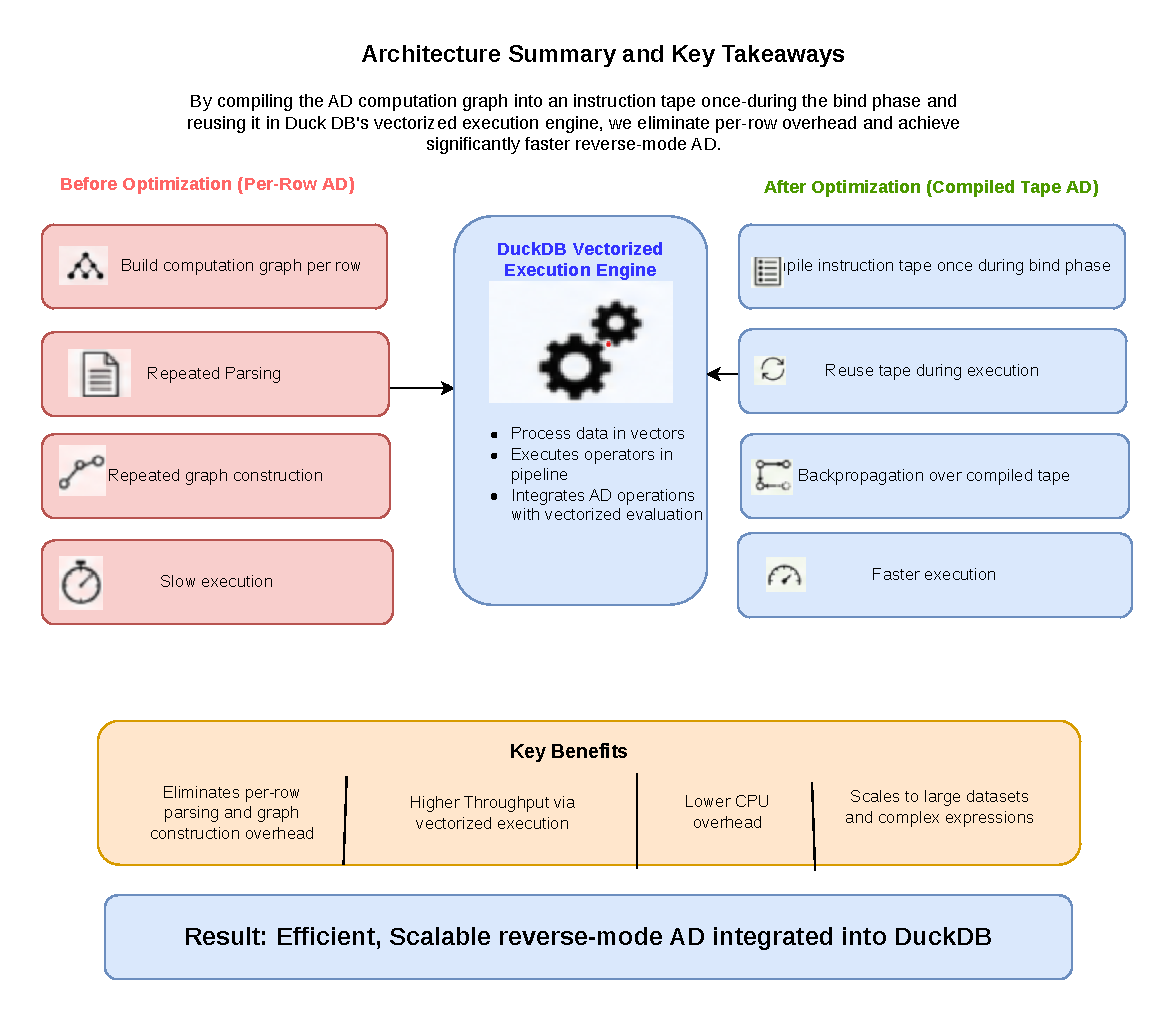
\includegraphics[width=\textwidth]{ad_summary.pdf}
\caption{Summary of the AD extension components added to DuckDB.}
\label{fig:ad-summary}
\end{figure}

The implementation demonstrated that automatic differentiation can be
integrated into a relational database system while reusing the existing
vectorized execution engine.

\section{Interpretation of Results}

The experimental evaluation compared three approaches for computing
gradients in a linear-regression gradient-descent workload: handwritten
SQL gradient expressions, forward-mode AD, and reverse-mode AD.

The handwritten SQL baseline consistently achieved the lowest runtime
across all dataset sizes. This was expected, since the gradients are
pre-derived by hand and execute as fused arithmetic expressions over
whole column vectors, so no abstraction or graph-construction overhead
is introduced during execution.

Forward-mode AD produced the highest runtimes among the evaluated
methods. In the implemented design, every intermediate value
propagates a complete gradient vector alongside the primal value, so
the amount of derivative propagation grows with the number of
parameters and the cost grows correspondingly with dataset size. The
bind-time operator-resolution optimization described in
Chapter~\ref{ch:implementation} substantially reduced this cost by
eliminating per-row string-based operator dispatch, but forward-mode
AD remains the slowest of the three methods because the per-operation
gradient propagation cost is intrinsic to the algorithm.

Reverse-mode AD performed substantially better than forward-mode AD
because its cost depends primarily on the number of operations in the
expression rather than on the number of parameters, which is consistent
with the standard complexity analysis in Appendix~\ref{app:proofs}.
Reverse-mode AD also stayed close to the handwritten baseline across
all dataset sizes. At 50{,}000 tuples the three methods required
approximately 0.11~seconds (baseline), 0.24~seconds (reverse-mode AD),
and 1.47~seconds (forward-mode AD). The relative behaviour is more
informative than these absolute figures: the advantage of reverse-mode
AD over forward-mode AD widens with scale, from roughly $1.5\times$
at 1{,}000 tuples to roughly $6.1\times$ at 50{,}000 tuples, while
reverse-mode AD stays within roughly $1.3\times$ to $2.2\times$ of the
handwritten baseline. Both trends are consistent with the design of
the three methods. The remaining gap between reverse-mode AD and the
baseline is attributable mainly to the fact that the tape is replayed
one row at a time within each chunk, whereas the handwritten baseline
executes as fused arithmetic that DuckDB's vectorized engine evaluates
across an entire column vector using SIMD-style
optimizations~\cite{kersten2018vectorized}.

\section{Effect of Tape Compilation}

One of the most important design choices in the reverse-mode implementation
was instruction tape reuse. A straightforward implementation of reverse-mode AD
would reconstruct the computation graph each time the lambda expression is
evaluated; because evaluation occurs once per row, this would place graph
construction directly on the per-row execution path. The implemented design
avoids this by exploiting an asymmetry in DuckDB's query pipeline: the
expression tree is compiled into a reusable instruction tape during the bind
phase, the compiled tape is stored in the function bind data, and only the
primal and adjoint values are updated for each row. Binding occurs exactly once
per query whereas execution occurs once per row, so this transformation reduces
tape construction from $N \cdot I$ times (for $N$ rows and $I$ gradient-descent
iterations) to a single time. This separation of a one-time compilation step
from repeated execution mirrors the strategy used by modern query compilers,
which specialize a query plan once and then execute the compiled form many
times~\cite{neumann2011efficiently,shaikhha2016compiler}. By construction, this
keeps repeated graph construction off the per-row execution path; a controlled
ablation isolating its quantitative effect is identified as future work.

\section{Answers to Research Questions}

This section revisits the research questions introduced in
Chapter~\ref{ch:introduction}.

\subsection*{RQ1: Can higher-order SQL lambda expressions be used to represent
differentiable computations inside DuckDB?}

Yes. Higher-order SQL lambda expressions were successfully used to represent
differentiable computations inside DuckDB. During binding, the lambda
expression body was extracted and converted into an internal representation
used for gradient computation.

\subsection*{RQ2: How can forward-mode and reverse-mode automatic
differentiation be integrated into DuckDB's query execution pipeline?}

Both differentiation modes were integrated using DuckDB's scalar function
infrastructure. Forward-mode AD propagated dual-number derivatives through the
expression tree during execution. Reverse-mode AD compiled the expression into
an instruction tape and executed adjoint propagation during a backward pass.
Both modes return the full gradient of the lambda expression in a single call,
as a structured value holding one partial derivative per argument. The
implementation reused DuckDB's existing vectorized execution engine and
required only localized modifications to the scalar function framework.

\subsection*{RQ3: Can reverse-mode AD be optimized using bind-time tape
compilation and reuse?}

Yes. The reverse-mode implementation compiles the instruction tape during the
binding phase and reuses it during execution. Because binding occurs once per
query rather than once per row, the tape is built a single time and replayed
for every row. By construction, this keeps repeated graph construction off the
per-row execution path. A controlled ablation measuring its isolated
quantitative effect against a per-row-rebuild baseline was outside the scope
of this work and is identified as future work.

\subsection*{RQ4: What performance overhead is introduced by automatic
differentiation inside SQL queries?}

The experiments showed that automatic differentiation introduces
measurable runtime overhead compared to handwritten SQL gradients.
The relative behaviour is consistent across dataset sizes: reverse-mode
AD substantially reduced overhead compared to forward-mode
differentiation, by a factor that grew from roughly $1.5\times$ at
1{,}000 tuples to roughly $6.1\times$ at 50{,}000 tuples, and stayed
within roughly $1.3\times$ to $2.2\times$ of handwritten SQL.The bind-time operator-resolution optimization in forward-mode AD removed per-row string-based operator dispatch and substantially reduced forward-mode runtime relative to an earlier variant without the optimization. Handwritten
SQL remained the fastest approach overall; the measured slowdown for
reverse-mode AD is the modest cost of replacing manual gradient
derivation with automatic differentiation.

\subsection*{RQ5: Can vectorized execution in DuckDB efficiently support
gradient computation over relational data?}

Yes, with a caveat. The implementation integrated with DuckDB's chunk-based
\texttt{DataChunk} execution model without requiring major modifications to the
query engine. The AD functions are invoked once per data chunk and reuse
DuckDB's execution infrastructure. Within each chunk, however, the instruction
tape is replayed one row at a time rather than evaluated across a whole column
vector; fully vectorizing the tape replay is identified as future work below.

\section{Limitations}

Although the implementation achieved the main objectives of the thesis,
several limitations remain. The current system supports only a limited subset
of arithmetic operators: addition, subtraction, multiplication, division, and
unary negation. Advanced mathematical operations such as exponential
functions, logarithms, trigonometric functions, and matrix operations were not
implemented. Reverse-mode differentiation supports only scalar-output lambda
expressions and does not support advanced SQL operations such as aggregations
or window functions.

In addition, the instruction tape is interpreted one row at a time rather
than vectorized across column vectors. This is the main remaining performance
gap relative to the handwritten baseline, and a vectorized tape interpreter
would be expected to narrow that gap. Finally, the experimental evaluation
considered only a single workload --- linear regression with squared loss ---
on a single hardware configuration, so the reported performance ratios should
not be assumed to generalize to all differentiable workloads.

\section{Future Work}

Several directions can extend this work in the future:

\begin{itemize}
  \item Support for additional mathematical operators such as logarithms,
        exponentials, and trigonometric functions.
  \item Differentiation through SQL aggregation and window functions.
  \item A vectorized tape interpreter that evaluates AD operations across
        whole column vectors rather than per row, for both forward-mode and
        reverse-mode AD. This is the main remaining performance gap relative
        to the handwritten baseline, since the current implementation
        replays the AD program one row at a time while the baseline executes
        as fused arithmetic across whole column vectors.
  \item Further optimization of forward-mode AD through bind-time
        specialisation of the gradient propagation loop. The current
        bind-time operator-resolution optimization removes string-based
        dispatch from the per-row path; a deeper specialisation could
        compile the forward-mode expression into a flat instruction
        sequence analogous to the reverse-mode tape, eliminating recursive
        function calls during evaluation.
  \item A controlled ablation measuring the isolated performance effect of
        bind-time tape compilation, by comparing the implemented design
        against a variant that reconstructs the computation graph per row.
  \item Support for vector-valued lambda expressions, rather than only            scalar outputs.
  \item Support for higher-order derivatives, such as Hessian-vector
        products~\cite{pearlmutter1994hessian}, to enable second-order
        optimization methods.
  \item Support for more complex machine learning workloads beyond linear
        regression.
  \item Integration through DuckDB's extension API instead of direct source
        modifications.
  \item Improved memory optimization for reverse-mode tape storage.
\end{itemize}

Future work may also explore integrating differentiable query execution with
distributed database systems and larger analytical workloads.

\section{Final Remarks}

This thesis demonstrated that automatic differentiation can be integrated
directly into DuckDB using higher-order SQL lambda expressions. The
implementation showed that reverse-mode automatic differentiation combined
with bind-time tape compilation significantly reduces differentiation overhead
compared to forward-mode approaches, that this advantage grows with dataset
size, and that reverse-mode AD stays within a small, near-constant factor of
handwritten SQL.

Although handwritten SQL gradients remain marginally faster, the proposed
system provides greater flexibility and automation while remaining fully
integrated within the relational database engine. The measured slowdown is the
modest cost of replacing manual gradient derivation with automatic
differentiation. The results suggest that differentiable database systems are
a promising approach for database-integrated gradient computation in future
analytical and machine learning workloads.

\appendix


%%%%%%%%%%%%%%%%%%%%%%%%%%%%%%%%%%%%%%%%%%%%%%%%%%%%
% APPENDIX A
%%%%%%%%%%%%%%%%%%%%%%%%%%%%%%%%%%%%%%%%%%%%%%%%%%%%

\chapter{Additional Implementation Details}
\label{app:implementation}

This appendix provides additional technical details regarding the implementation of automatic differentiation inside DuckDB. The material included here supplements the implementation discussion presented in Chapter~\ref{ch:implementation}.

%------------------------------------------------

\section{Complete Forward-Mode AD Implementation}

The forward-mode AD system is implemented using dual-number propagation. Each scalar value is extended with a gradient vector that is propagated through arithmetic operations during expression evaluation.

The core structure used inside DuckDB is:

\begin{lstlisting}[language=C++]
struct Dual {
    double val;
    std::vector<double> grad;
};
\end{lstlisting}

The multiplication operator propagates derivatives according to the product rule:

\[
(a \cdot b)' = a'b + ab'
\]

\begin{lstlisting}[language=C++]
Dual multiply(const Dual &a, const Dual &b) {
    Dual out;

    out.val = a.val * b.val;
    out.grad.resize(a.grad.size());

    for (size_t i = 0; i < out.grad.size(); i++) {
        out.grad[i] =
            a.grad[i] * b.val +
            b.grad[i] * a.val;
    }

    return out;
}
\end{lstlisting}

Additional operator overloads were implemented for addition, subtraction, division, unary negation, and scalar constants.

%------------------------------------------------

\section{Reverse-Mode Tape Structure}

Reverse-mode AD uses a reusable instruction tape generated during the bind phase. The tape is a single contiguous array of operations, indexed by integer position rather than traversed through pointers. Each operation stores its operation kind and the indices of its operand operations:

\begin{lstlisting}[language=C++]
struct CompiledOp {
    OpKind  op;          // INPUT, CONST, NEG, ADD, SUB, MUL, DIV
    int32_t a, b;        // operand indices into the program
    double  cval;        // constant value (CONST only)
    int32_t input_slot;  // parameter slot (INPUT only)
};
\end{lstlisting}

The primal values and adjoint values are not stored inside the operation records. Instead, they are held in two separate working buffers, each the size of the tape, which are allocated once per data chunk and reused for every row.

The tape is executed in two stages:

\begin{enumerate}
    \item a forward pass, which evaluates the operations in order and stores their primal values;
    \item a reverse pass, which traverses the operations in reverse order and accumulates adjoint values into each operand.
\end{enumerate}

The binder compiles the tape once and stores it in the function bind data for reuse during vectorized execution.

%------------------------------------------------

\section{Tape Compilation Algorithm}

The following pseudocode illustrates binder-time tape generation. Each call appends one operation to the program and returns its index, so that parent operations can reference their operands by position:

\begin{lstlisting}
function CompileTape(expr):

    if expr is constant:
        return EmitConst(expr.value)

    if expr is variable:
        return EmitInput(expr.slot)

    if expr is unary negation:
        a = CompileTape(expr.child)
        return EmitNeg(a)

    left  = CompileTape(expr.left)
    right = CompileTape(expr.right)
    return EmitBin(expr.op, left, right)
\end{lstlisting}

Because this compilation runs once during binding, it eliminates repeated graph construction during query execution.

%%%%%%%%%%%%%%%%%%%%%%%%%%%%%%%%%%%%%%%%%%%%%%%%%%%%
% APPENDIX B
%%%%%%%%%%%%%%%%%%%%%%%%%%%%%%%%%%%%%%%%%%%%%%%%%%%%

\chapter{Extended Experimental Results}
\label{app:experiments}

This appendix presents additional benchmark results and raw experimental data used in the evaluation chapter.

%------------------------------------------------

\section{Complete Runtime Measurements}

Table~\ref{tab:extended_runtime} shows the median execution times for all benchmark configurations, measured on the optimized release build over five runs per configuration.

\begin{table}[H]
\centering
\begin{tabular}{|c|c|c|c|}
\hline
Rows & Baseline & Forward AD & Reverse AD \\
\hline
1,000  & 0.03 s & 0.06 s & 0.04 s \\
5,000  & 0.05 s & 0.21 s & 0.05 s \\
10,000 & 0.04 s & 0.32 s & 0.07 s \\
20,000 & 0.06 s & 0.70 s & 0.13 s \\
50,000 & 0.11 s & 1.47 s & 0.24 s \\
\hline
\end{tabular}
\caption{Extended runtime benchmark results (optimized release build, median of five runs, single-threaded).}
\label{tab:extended_runtime}
\end{table}

The raw per-run measurements underlying this table were recorded in a comma-separated file with one row per dataset size, method, and repetition. A separate aggregation step computed the median, minimum, and maximum per configuration and wrote a summary file used directly as the input table for the plots in Chapter~\ref{ch:evaluation}.

%------------------------------------------------

\section{Additional SQL Benchmark Queries}

In the benchmark queries, the AD function receives the numeric arguments first and the lambda expression last. The lambda declares one parameter per numeric argument, in the same positional order. The function returns a structured value holding one partial derivative per argument; the derivatives with respect to the trainable parameters are read from the corresponding struct fields.

Example forward-mode query:

\begin{lstlisting}[language=SQL]
SELECT mygrad_fwd(
    w, b, x, y,
    (p1, p2, p3, p4) ->
        (p1 * p3 + p2 - p4) *
        (p1 * p3 + p2 - p4)
)
FROM data;
\end{lstlisting}

Example reverse-mode query:

\begin{lstlisting}[language=SQL]
SELECT mygrad_rev(
    w, b, x, y,
    (p1, p2, p3, p4) ->
        (p1 * p3 + p2 - p4) *
        (p1 * p3 + p2 - p4)
)
FROM data;
\end{lstlisting}

%------------------------------------------------

\section{Effect of Tape Reuse}

A straightforward implementation of reverse-mode AD would rebuild the
computation graph for every processed tuple, placing graph construction on the
per-row execution path. The implemented design instead compiles the tape once,
during binding, stores it in the function bind data, and reuses it across all
rows. Figure~\ref{fig:tape_reuse} illustrates this difference.

\begin{figure}[H]
\centering
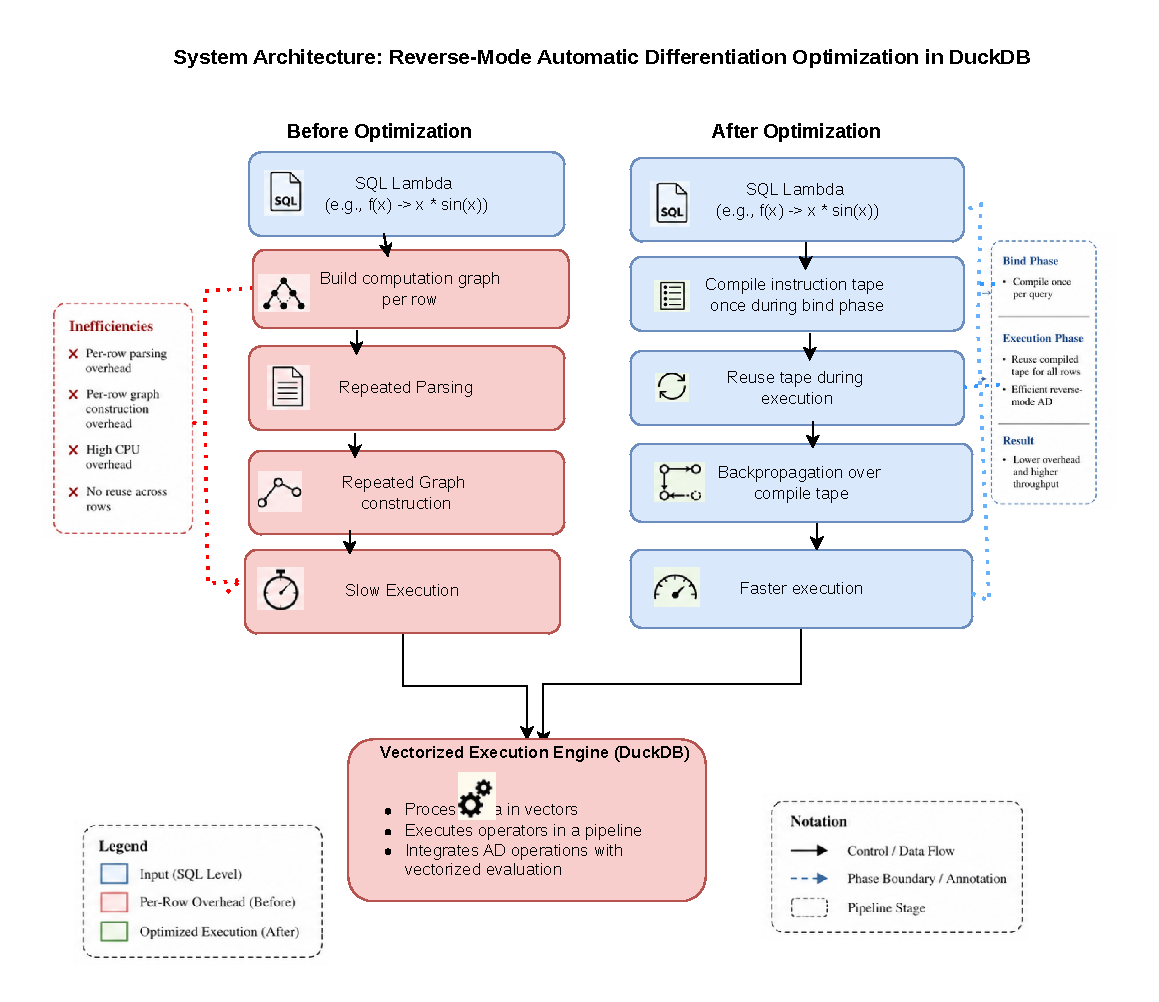
\includegraphics[width=\textwidth]{tape_reuse.pdf}
\caption{Performance benefit of instruction tape reuse in reverse-mode AD.}
\label{fig:tape_reuse}
\end{figure}

In summary, the implemented design:
\begin{itemize}
    \item compiles the tape once during binding,
    \item stores the compiled tape in the function bind data,
    \item reuses it for every row across all data chunks.
\end{itemize}
By construction, this keeps repeated graph construction off the per-row
execution path. A measured before/after comparison against a per-row-rebuild
variant is identified as future work in Chapter~\ref{ch:conclusion}.

%%%%%%%%%%%%%%%%%%%%%%%%%%%%%%%%%%%%%%%%%%%%%%%%%%%%
% APPENDIX C
%%%%%%%%%%%%%%%%%%%%%%%%%%%%%%%%%%%%%%%%%%%%%%%%%%%%

\chapter{Mathematical Foundations}
\label{app:proofs}

This appendix provides mathematical derivations and correctness arguments for the implemented automatic differentiation algorithms.

%------------------------------------------------

\section{Correctness of Forward-Mode AD}

Forward-mode AD propagates derivatives using the chain rule. For a composition

\[
f(x) = g(h(x))
\]

the derivative is

\[
f'(x) = g'(h(x)) \cdot h'(x).
\]

The implemented dual-number propagation preserves this property for every primitive operator. For multiplication,

\[
f(x) = u(x)\,v(x),
\]

the derivative rule is

\[
f'(x) = u'(x)\,v(x) + u(x)\,v'(x),
\]

which matches the implemented operator logic shown in Appendix~\ref{app:implementation}.

%------------------------------------------------

\section{Complexity Analysis}

Let $n$ denote the number of operations in the compiled expression and $p$ the number of parameters.

Forward-mode AD propagates a gradient vector of length $p$ alongside each of the $n$ intermediate values, giving a time complexity of

\[
O(n \cdot p).
\]

Reverse-mode AD evaluates the tape with a single forward pass and a single reverse pass, each linear in the number of operations, giving a time complexity of

\[
O(n)
\]

for scalar-output functions, independent of the number of parameters. Its memory complexity is also O(n) per row, due to the storage of intermediate primal values and adjoints; in the implementation, these buffers are allocated once per data chunk and reused across rows within the chunk. These asymptotic characteristics are consistent with the standard analysis of forward- and reverse-mode AD given by Griewank and Walther~\cite{griewank2008evaluating} and Baydin et al.~\cite{baydin2017automatic}.

These complexity characteristics explain why reverse-mode AD outperforms forward-mode AD for workloads with many parameters, and they are consistent with the experimental results in Chapter~\ref{ch:evaluation}, where the advantage of reverse-mode AD over forward-mode AD widens as the workload grows.


%%%%%%%%%%%%%%%%%%%%%%%%%%%%%%%%%%%%%%%%%%%%%%%%%%%%
% BIBLIOGRAPHY
%%%%%%%%%%%%%%%%%%%%%%%%%%%%%%%%%%%%%%%%%%%%%%%%%%%%

\newpage

\begin{thebibliography}{99}

\bibitem{baydin2017automatic}
Baydin, Atilim G{\"u}ne{\c{s}}, Barak A. Pearlmutter, Alexey Andreyevich Radul, and Jeffrey Mark Siskind (2017).
``Automatic Differentiation in Machine Learning: A Survey''.
\textit{Journal of Machine Learning Research} 18,
153:1--153:43.

\bibitem{griewank2008evaluating}
Griewank, Andreas and Andrea Walther (2008).
\textit{Evaluating Derivatives: Principles and Techniques of Algorithmic Differentiation}.
Second Edition.
Philadelphia, PA, USA: SIAM.
ISBN: 978-0-89871-659-7.

\bibitem{jax2018}
Bradbury, James, Roy Frostig, Peter Hawkins,
Matthew James Johnson, Yash Katariya, Chris Leary,
Dougal Maclaurin, George Necula, Adam Paszke,
Jake VanderPlas, Skye Wanderman-Milne, and Qiao Zhang (2018).
\textit{JAX: Composable Transformations of Python+NumPy Programs}.
Software library.
\url{https://github.com/jax-ml/jax}.

\bibitem{abadi2016tensorflow}
Abadi, Mart\'in, Paul Barham, Jianmin Chen, Zhifeng Chen, Andy Davis,
Jeffrey Dean, Matthieu Devin, Sanjay Ghemawat, Geoffrey Irving,
Michael Isard, Manjunath Kudlur, Josh Levenberg, Rajat Monga,
Sherry Moore, Derek Gordon Murray, Benoit Steiner, Paul A. Tucker,
Vijay Vasudevan, Pete Warden, Martin Wicke, Yuan Yu, and Xiaoqiang Zheng (2016).
``TensorFlow: A System for Large-Scale Machine Learning''.
In: \textit{Proceedings of the 12th USENIX Symposium on Operating Systems Design and Implementation (OSDI)},
pp.~265--283.

\bibitem{paszke2019pytorch}
Paszke, Adam, Sam Gross, Francisco Massa, Adam Lerer,
James Bradbury, Gregory Chanan, Trevor Killeen,
Zeming Lin, Natalia Gimelshein, Luca Antiga,
Alban Desmaison, Andreas K{\"o}pf, Edward Z. Yang,
Zachary DeVito, Martin Raison, Alykhan Tejani,
Sasank Chilamkurthy, Benoit Steiner, Lu Fang,
Junjie Bai, and Soumith Chintala (2019).
``PyTorch: An Imperative Style, High-Performance Deep Learning Library''.
In: \textit{Advances in Neural Information Processing Systems (NeurIPS)},
Vol.~32, pp.~8024--8035.


\bibitem{duckdb2019}
Raasveldt, Mark and Hannes M{\"u}hleisen (2019).
``DuckDB: An Embeddable Analytical Database''.
In: \textit{Proceedings of the 2019 International Conference on Management of Data (SIGMOD)},
pp.~1981--1984.

\bibitem{raasveldt2022modular}
Raasveldt, Mark (2022).
``DuckDB -- A Modern Modular and Extensible Database System''.
In: \textit{CDMS Workshop at VLDB}.


\bibitem{schikuta2008neural}
Schikuta, Erich (2008).
``Neural Networks and Database Systems''.
In: \textit{arXiv preprint arXiv:0802.3582}.

\bibitem{baudart2021stan}
Baudart, Guillaume, Javier Burroni, Martin Hirzel,
Louis Mandel, and Avraham Shinnar (2021).
``Compiling Stan to Generative Probabilistic Languages and Extension to Deep Probabilistic Programming''.
In: \textit{Proceedings of the ACM SIGPLAN Conference on Programming Language Design and Implementation (PLDI)},
pp.~497--510.

\bibitem{innes2018adjoint}
Innes, Michael (2018).
``Don't Unroll Adjoint: Differentiating SSA-Form Programs''.
In: \textit{CoRR}, abs/1810.07951.

\bibitem{chen2015mxnet}
Chen, Tianqi, Mu Li, Yutian Li, Min Lin,
Naiyan Wang, Minjie Wang, Tianjun Xiao,
Bing Xu, Chiyuan Zhang, and Zheng Zhang (2015).
``MXNet: A Flexible and Efficient Machine Learning Library for Heterogeneous Distributed Systems''.
In: \textit{CoRR}, abs/1512.01274.

\bibitem{agrawal2019eager}
Agrawal, Akshay, Akshay Naresh Modi,
Alexandre Passos, Allen Lavoie,
Ashish Agarwal, Asim Shankar,
Igor Ganichev, Josh Levenberg,
Mingsheng Hong, Rajat Monga,
and Shanqing Cai (2019).
``TensorFlow Eager: A Multi-Stage, Python-Embedded DSL for Machine Learning''.
In: \textit{Proceedings of SysML}.

\bibitem{boehm2013systemml}
Boehm, Matthias, Douglas Burdick,
Alexandre V. Evfimievski, Berthold Reinwald,
Prithviraj Sen, Shirish Tatikonda,
and Yuanyuan Tian (2013).
``Compiling Machine Learning Algorithms with SystemML''.
In: \textit{Proceedings of the ACM Symposium on Cloud Computing (SoCC)},
Article 57.

\bibitem{meng2016mllib}
Meng, Xiangrui, Joseph K. Bradley, Burak Yavuz,
Evan Randall Sparks, Shivaram Venkataraman,
Davies Liu, Jeremy Freeman, D. B. Tsai,
Manish Amde, Sean Owen, Doris Xin,
Reynold Xin, Michael J. Franklin,
Reza Zadeh, Matei Zaharia, and Ameet Talwalkar (2016).
``MLlib: Machine Learning in Apache Spark''.
In: \textit{Journal of Machine Learning Research} 17(34),
pp.~1--7.

\bibitem{zaharia2016spark}
Zaharia, Matei, Reynold S. Xin, Patrick Wendell,
Tathagata Das, Michael Armbrust, Ankur Dave,
Xiangrui Meng, Josh Rosen, Shivaram Venkataraman,
Michael J. Franklin, Ali Ghodsi, Joseph Gonzalez,
Scott Shenker, and Ion Stoica (2016).
``Apache Spark: A Unified Engine for Big Data Processing''.
In: \textit{Communications of the ACM} 59(11),
pp.~56--65.


\bibitem{stonebraker2013voltdb}
Stonebraker, Michael and Ariel Weisberg (2013).
``The VoltDB Main Memory DBMS''.
In: \textit{IEEE Data Engineering Bulletin} 36(2),
pp.~21--27.

\bibitem{neumann2011efficiently}
Neumann, Thomas (2011).
``Efficiently Compiling Efficient Query Plans for Modern Hardware''.
In: \textit{Proceedings of the VLDB Endowment} 4(9),
pp.~539--550.

\bibitem{boncz2008monetdb}
Boncz, Peter A., Martin L. Kersten,
and Stefan Manegold (2008).
``Breaking the Memory Wall in MonetDB''.
In: \textit{Communications of the ACM} 51(12),
pp.~77--85.

\bibitem{harizopoulos2008oltp}
Harizopoulos, Stavros, Daniel J. Abadi,
Samuel Madden, and Michael Stonebraker (2008).
``OLTP Through the Looking Glass, and What We Found There''.
In: \textit{Proceedings of the 2008 ACM SIGMOD International Conference on Management of Data},
pp.~981--992.

\bibitem{graefe1994volcano}
Graefe, Goetz (1994).
``Volcano --- An Extensible and Parallel Query Evaluation System''.
In: \textit{IEEE Transactions on Knowledge and Data Engineering} 6(1),
pp.~120--135.


\bibitem{kraska2018learned}
Kraska, Tim, Alex Beutel, Ed H. Chi,
Jeffrey Dean, and Neoklis Polyzotis (2018).
``The Case for Learned Index Structures''.
In: \textit{Proceedings of the 2018 ACM SIGMOD International Conference on Management of Data},
pp.~489--504.

\bibitem{peseux2023differentiable}
Peseux, Paul (2023).
\textit{Programmation Diff\'erentiable \`a Grande \'Echelle pour les Donn\'ees Relationnelles
(A Differentiable Programming Approach for Optimization on Relational and Large Datasets)}.
Normandy University, Caen, France.

\bibitem{payani2020relational}
Payani, Ali and Faramarz Fekri (2020).
``Incorporating Relational Background Knowledge into Reinforcement Learning via Differentiable Inductive Logic Programming''.
In: \textit{CoRR}, abs/2003.10386.

\bibitem{tahboub2018compiler}
Tahboub, Ruby Y., Gr\'egory M. Essertel,
and Tiark Rompf (2018).
``How to Architect a Query Compiler, Revisited''.
In: \textit{Proceedings of the 2018 ACM SIGMOD International Conference on Management of Data},
pp.~307--322.

\bibitem{shaikhha2016compiler}
Shaikhha, Amir, Yannis Klonatos,
Lionel Parreaux, Lewis Brown,
Mohammad Dashti, and Christoph Koch (2016).
``How to Architect a Query Compiler''.
In: \textit{Proceedings of the 2016 ACM SIGMOD International Conference on Management of Data},
pp.~1907--1922.

\bibitem{cheung2013synthesis}
Cheung, Alvin, Armando Solar-Lezama,
and Samuel Madden (2013).
``Optimizing Database-Backed Applications with Query Synthesis''.
In: \textit{Proceedings of the ACM SIGPLAN Conference on Programming Language Design and Implementation (PLDI)},
pp.~3--14.


\bibitem{kohn2022duckdbwasm}
Kohn, Andr\'e, Dominik Moritz,
Mark Raasveldt, Hannes M{\"u}hleisen,
and Thomas Neumann (2022).
``DuckDB-Wasm: Fast Analytical Processing for the Web''.
In: \textit{Proceedings of the VLDB Endowment} 15(12),
pp.~3574--3577.

\bibitem{boehm2016systemml}
Boehm, Matthias, Michael Dusenberry,
Deron Eriksson, Alexandre V. Evfimievski,
Faraz Makari Manshadi, Niketan Pansare,
Berthold Reinwald, Frederick Reiss,
Prithviraj Sen, Arvind Surve,
and Shirish Tatikonda (2016).
``SystemML: Declarative Machine Learning on Spark''.
In: \textit{Proceedings of the VLDB Endowment} 9(13),
pp.~1425--1436.

\bibitem{chen2018tvm}
Chen, Tianqi, Thierry Moreau,
Ziheng Jiang, Lianmin Zheng,
Eddie Q. Yan, Haichen Shen,
Meghan Cowan, Leyuan Wang,
Yuwei Hu, Luis Ceze,
Carlos Guestrin, and Arvind Krishnamurthy (2018).
``TVM: An Automated End-to-End Optimizing Compiler for Deep Learning''.
In: \textit{Proceedings of OSDI},
pp.~578--594.

\bibitem{chen2024glo}
Chen, Tianyi, Jun Gao,
Yaofeng Tu, and Mo Xu (2024).
``GLO: Towards Generalized Learned Query Optimization''.
In: \textit{Proceedings of ICDE},
pp.~4843--4855.

\bibitem{pavlo2017selfdriving}
Pavlo, Andrew, Gustavo Angulo,
Joy Arulraj, Haibin Lin,
Jiexi Lin, Lin Ma,
Prashanth Menon, Todd C. Mowry,
Matthew Perron, Ian Quah,
Siddharth Santurkar, Anthony Tomasic,
Skye Toor, Dana Van Aken,
Ziqi Wang, Yingjun Wu,
Ran Xian, and Tieying Zhang (2017).
``Self-Driving Database Management Systems''.
In: \textit{CIDR}.

\bibitem{codd1970relational}
Codd, E. F. (1970).
``A Relational Model of Data for Large Shared Data Banks''.
In: \textit{Communications of the ACM} 13(6),
pp.~377--387.


\bibitem{selinger1979access}
Selinger, Patricia G., Morton M. Astrahan,
Donald D. Chamberlin, Raymond A. Lorie,
and Thomas G. Price (1979).
``Access Path Selection in a Relational Database Management System''.
In: \textit{Proceedings of the 1979 ACM SIGMOD International Conference on Management of Data},
pp.~23--34.


\bibitem{pearlmutter1994hessian}
Pearlmutter, Barak A. (1994).
``Fast Exact Multiplication by the Hessian''.
In: \textit{Neural Computation} 6(1),
pp.~147--160.

\bibitem{grum2023backprop}
Grum, Marcus (2023).
``Learning Representations by Crystallized Back-Propagating Errors''.
In: \textit{ICAISC},
pp.~78--100.

\bibitem{kingma2015adam}
Kingma, Diederik P. and Jimmy Ba (2015).
``Adam: A Method for Stochastic Optimization''.
In: \textit{ICLR}.

\bibitem{maclaurin2015reversible}
Maclaurin, Dougal, David Duvenaud,
and Ryan P. Adams (2015).
``Gradient-Based Hyperparameter Optimization through Reversible Learning''.
In: \textit{Proceedings of ICML},
pp.~2113--2122.


\bibitem{dean2004mapreduce}
Dean, Jeffrey and Sanjay Ghemawat (2004).
``MapReduce: Simplified Data Processing on Large Clusters''.
In: \textit{Proceedings of OSDI},
pp.~137--150.

\bibitem{zaharia2012rdd}
Zaharia, Matei, Mosharaf Chowdhury,
Tathagata Das, Ankur Dave,
Justin Ma, Murphy McCauly,
Michael J. Franklin, Scott Shenker,
and Ion Stoica (2012).
``Resilient Distributed Datasets: A Fault-Tolerant Abstraction for In-Memory Cluster Computing''.
In: \textit{Proceedings of NSDI},
pp.~15--28.


\bibitem{armbrust2015sparksql}
Armbrust, Michael, Reynold S. Xin, Cheng Lian, Yin Huai,
Davies Liu, Joseph K. Bradley, Xiangrui Meng,
Tomer Kaftan, Michael J. Franklin, Ali Ghodsi,
and Matei Zaharia (2015).
``Spark SQL: Relational Data Processing in Spark''.
In: \textit{Proceedings of the 2015 ACM SIGMOD International Conference on Management of Data},
pp.~1383--1394.

\bibitem{stonebraker2005cstore}
Stonebraker, Michael, Daniel J. Abadi,
Adam Batkin, Xuedong Chen,
Mitch Cherniack, Miguel Ferreira,
Edmond Lau, Amerson Lin,
Samuel Madden, Elizabeth J. O'Neil,
Patrick E. O'Neil, Alex Rasin,
Nga Tran, and Stanley B. Zdonik (2005).
``C-Store: A Column-Oriented DBMS''.
In: \textit{Proceedings of VLDB},
pp.~553--564.

\bibitem{hubner2011differential}
H{\"u}bner, Florian, Joos-Hendrik B{\"o}se,
Jens Kr{\"u}ger, Cafer Tosun,
Alexander Zeier, and Hasso Plattner (2011).
``A Cost-Aware Strategy for Merging Differential Stores in Column-Oriented In-Memory DBMS''.
In: \textit{BIRTE},
pp.~38--52.


\bibitem{abadi2006compression}
Abadi, Daniel J., Samuel Madden,
and Miguel Ferreira (2006).
``Integrating Compression and Execution in Column-Oriented Database Systems''.
In: \textit{Proceedings of the 2006 ACM SIGMOD International Conference on Management of Data},
pp.~671--682.


\bibitem{harizopoulos2006readoptimized}
Harizopoulos, Stavros, Velen Liang,
Daniel J. Abadi, and Samuel Madden (2006).
``Performance Tradeoffs in Read-Optimized Databases''.
In: \textit{Proceedings of VLDB},
pp.~487--498.

\bibitem{hyper2011}
Kemper, Alfons and Thomas Neumann (2011).
``HyPer: A Hybrid OLTP\&OLAP Main Memory Database System Based on Virtual Memory Snapshots''.
In: \textit{ICDE},
pp.~195--206.

\bibitem{leis2014morsel}
Leis, Viktor et al. (2014).
``Morsel-Driven Parallelism: A NUMA-Aware Query Evaluation Framework for the Many-Core Age''.
In: \textit{SIGMOD},
pp.~743--754.

\bibitem{graefe1993query}
Graefe, Goetz (1993).
``Query Evaluation Techniques for Large Databases''.
In: \textit{ACM Computing Surveys} 25(2),
pp.~73--170.

\bibitem{chaudhuri1998optimization}
Chaudhuri, Surajit (1998).
``An Overview of Query Optimization in Relational Systems''.
In: \textit{Proceedings of PODS},
pp.~34--43.

\bibitem{abouzeid2009hadoopdb}
Abouzeid, Azza, Kamil Bajda-Pawlikowski,
Daniel J. Abadi, Alexander Rasin,
and Avi Silberschatz (2009).
``HadoopDB: An Architectural Hybrid of MapReduce and DBMS Technologies for Analytical Workloads''.
In: \textit{Proceedings of the VLDB Endowment} 2(1),
pp.~922--933.

\bibitem{manegold2002mainmemory}
Manegold, Stefan, Peter Boncz,
and Martin L. Kersten (2002).
``Optimizing Main-Memory Join on Modern Hardware''.
In: \textit{IEEE Transactions on Knowledge and Data Engineering} 14(4),
pp.~709--730.

\bibitem{kersten2018vectorized}
Kersten, Timo, Viktor Leis,
Alfons Kemper, Thomas Neumann,
Andrew Pavlo, and Peter Boncz (2018).
``Everything You Always Wanted to Know About Compiled and Vectorized Queries But Were Afraid to Ask''.
In: \textit{Proceedings of the VLDB Endowment} 11(13),
pp.~2209--2222.

\bibitem{pearlmutter2008reverse}
Pearlmutter, Barak A. and Jeffrey Mark Siskind (2008).
``Reverse-Mode AD in a Functional Framework: Lambda the Ultimate Backpropagator''.
In: \textit{ACM Transactions on Programming Languages and Systems} 30(2),
Article 7.

\bibitem{ribeiro2016trust}
Ribeiro, Marco T\'ulio, Sameer Singh,
and Carlos Guestrin (2016).
``Why Should I Trust You?: Explaining the Predictions of Any Classifier''.
In: \textit{Proceedings of the 22nd ACM SIGKDD International Conference on Knowledge Discovery and Data Mining},
pp.~1135--1144.

\bibitem{melnik2010dremel}
Melnik, Sergey, Andrey Gubarev,
Jing Jing Long, Geoffrey Romer,
Shiva Shivakumar, Matt Tolton,
and Theo Vassilakis (2010).
``Dremel: Interactive Analysis of Web-Scale Datasets''.
In: \textit{Proceedings of the VLDB Endowment} 3(1--2),
pp.~330--339.

\bibitem{olston2008piglatin}
Olston, Christopher, Benjamin C. Reed,
Utkarsh Srivastava, Ravi Kumar,
and Andrew Tomkins (2008).
``Pig Latin: A Not-So-Foreign Language for Data Processing''.
In: \textit{Proceedings of the 2008 ACM SIGMOD International Conference on Management of Data},
pp.~1099--1110.

\bibitem{madlib}
Hellerstein, Joseph M., Christopher R\'e, Florian Schoppmann,
Daisy Zhe Wang, Eugene Fratkin, Aleksander Gorajek,
Kee Siong Ng, Caleb Welton, Xixuan Feng,
Kun Li, and Arun Kumar (2012).
``The MADlib Analytics Library or MAD Skills, the SQL''.
In: \textit{Proceedings of the VLDB Endowment} 5(12),
pp.~1700--1711.

\bibitem{feng2012unified}
Feng, Xixuan, Arun Kumar, Benjamin Recht, and Christopher R\'e (2012).
``Towards a Unified Architecture for In-RDBMS Analytics''.
In: \textit{Proceedings of the 2012 ACM SIGMOD International Conference on Management of Data},
pp.~325--336.

\end{thebibliography}

%%%%%%%%%%%%%%%%%%%%%%%%%%%%%%%%%%%%%%%%%%%%%%%%%%%%
% DECLARATION
%%%%%%%%%%%%%%%%%%%%%%%%%%%%%%%%%%%%%%%%%%%%%%%%%%%%

\newpage

\chapter*{Declaration}
\addcontentsline{toc}{chapter}{Declaration}

In accordance with academic regulations and principles of good scientific
practice, I hereby declare that I have written the present master's thesis
entitled

\begin{center}
\textit{``Higher-Order SQL Lambda Functions in DuckDB''}
\end{center}

independently and solely by myself. All sources, references, and external
materials used in this thesis have been properly acknowledged and cited
where appropriate.

I further declare that this thesis has not previously been submitted,
either wholly or partially, for the award of any other degree, diploma,
or academic qualification at this or any other university or institution.

Generative AI tools were used only in a limited and supportive manner for
brainstorming, language refinement, grammar correction, formatting assistance,
and structural organization. The core research ideas, implementation,
experimental evaluation, technical analysis, architectural design, and
conclusions presented in this thesis are entirely my own original work.

Furthermore, I declare that the contents of both the digital and printed
versions of this thesis are identical. I understand that this thesis may
be subjected to plagiarism detection and software-assisted academic integrity
verification.

\vspace{4cm}

\noindent
\begin{minipage}{0.4\textwidth}
\centering
\rule{6cm}{0.4pt}\\
Date
\end{minipage}
\hfill
\begin{minipage}{0.4\textwidth}
\centering
\rule{6cm}{0.4pt}\\
Signature
\end{minipage}

\end{document}